%%%%%%%%%%%%%%%%%%%%%%%%%%%%%%%%%%%%%%%%%%%%%%%%%%%%%%%%%%%%%%%%%%%%%%%%
%    INSTITUTE OF PHYSICS PUBLISHING                                   %
%                                                                      %
%   `Preparing an article for publication in an Institute of Physics   %
%    Publishing journal using LaTeX'                                   %
%                                                                      %
%    LaTeX source code `ioplau2e.tex' used to generate `author         %
%    guidelines', the documentation explaining and demonstrating use   %
%    of the Institute of Physics Publishing LaTeX preprint files       %
%    `iopart.cls, iopart12.clo and iopart10.clo'.                      %
%                                                                      %
%    `ioplau2e.tex' itself uses LaTeX with `iopart.cls'                %
%                                                                      %
%%%%%%%%%%%%%%%%%%%%%%%%%%%%%%%%%%%%%%%%%%%%%%%%%%%%%%%%%%%%%%%%%%%%%%%%

% Document class definition
\documentclass[12pt]{iopart}

% Addition of neater URL's and hyperrefs
\usepackage{url} 

% better encoding of text
\usepackage[T1]{fontenc}

% Addition of linenumbers 
\usepackage{lineno} 
\linenumbers

% for nicer non-forced page breaks
\usepackage{afterpage}

% long tables
\usepackage{longtable}

% For nicer subfigures
\usepackage{subcaption}  

% A short-hand for superscripting
\newcommand{\ts}[1]{\textsuperscript{#1}}

% short-hand for the index name
\newcommand{\credi}[0]{{\sc credi}}
\newcommand{\sdi}[0]{{\sc solar credi}}
\newcommand{\wdi}[0]{{\sc wind credi}}

% nicer figures
\usepackage{graphicx}

%% Determine bibliography 
\usepackage[style=authoryear,backend=biber]{biblatex}
\addbibresource{sample.bib}


%% set section names for Supp. Info
% sections
\renewcommand\thesection{\Alph{section}}
\renewcommand\thesubsection{\thesection.\Alph{subsection}}
\renewcommand\thesubsubsection{\thesubsection.\Alph{subsubsection}}
% figures
\renewcommand\thefigure{SI.\arabic{figure}}    
\renewcommand\thetable{SI.\arabic{table}}    


% Start of the document
\begin{document}

% title
\title[Supp. Inf. to the Climatological Renewable Energy Deviation Index]{Supporting Information for the Climatological Renewable Energy Deviation Index}

% Author list
\author{Laurens P. Stoop$^{1,2,3,A}$, Karin van der Wiel$^{4,B}$, William Zappa$^{3,N}$, Arno Haverkamp$^{3,O}$, Ad J. Feelders$^{1,Y}$ and Machteld van den Broek$^{4,Z}$}

% Adresses
\address{$^1$ Information and Computing Science, Utrecht University, the Netherlands}
\address{$^2$ Copernicus Institute of Sustainable Development, Utrecht University, the Netherlands}
\address{$^3$ TenneT TSO B.V., Arnhem, the Netherlands}
\address{$^4$ Royal Netherlands Meteorological Institute (KNMI), the Netherlands}
\address{$^5$ Integrated Research on Energy, Environment and Society, Energy and Sustainability Research Institute Groningen (ESRIG), University of Groningen, the Netherlands}

% ORCiD list
\orcid{$^A$ 0000-0003-2756-5653}
\orcid{$^B$ 0000-0001-9365-5759}
\orcid{$^N$ 0000-0001-6810-7224}
\orcid{$^O$ 0000-0001-6947-7892}
\orcid{$^Y$ 0000-0003-4525-1949}
\orcid{$^Z$ 0000-0003-1028-1742}

% Contact information
\ead{l.p.stoop@uu.nl}
\vspace{10pt}
\begin{indented}
\item[]July 2023
\end{indented}

% Uncomment for Submitted to journal title message
\submitto{\ERL}
% ERL would mean 4000 words max

% Uncomment if a separate title page is required
\maketitle



%%%%%%%%%%%%%%%%%%%%%%%%%%%%%%%%%%%%%%%%%%%%%%%%%%
%%%%		~~~~ Comparison of Climate def ~~~~


\section{Comparison of Climatic Definitions of the Renewable Resources}
Section 2 in the main text describes the observed climatic behaviour of wind and solar energy potential and shows the use of the hourly rolling window climate for renewable resources. 
Here we provide some additional figures and analysis on the specific behaviour during each hour of the day (Section~\ref{app:clima_hourly}). 
We also highlight the use of different climate definitions (Section~\ref{app:Harmonics}) and discuss the sensitivity of the hourly rolling window climate on its window size (Section~\ref{app:sense}).

\subsection{Climatic characterisation for each hour of the day }\label{app:clima_hourly}
% motivation
Section 2.1 in the main text describes the observed variability of wind and solar energy potential. 
Here we provide some additional figures (Figure~\ref{SIfig:climate_solar_hourly} and \ref{SIfig:climate_wind_hourly}) show the climatic behaviour throughout the year, for each hour of the day separately. 

% Solar
For solar, the strong annual and diurnal cycle are very clearly visible. 
In addition, a few peculiarities can be observed related to how solar panels function. 
The efficiency of solar panels declines with increasing air temperature~\parencite{SaintDrenan2018}, leading to a reduced solar generation potential around noon after the summer solstice from the higher temperatures at this time of the year.  
\begin{figure}[b]
    \centering
    \includegraphics[width=\textwidth]{Figures_SI/climatology_solar_hourly.pdf}
    \caption{
    The climatological definitions for the solar potential generation is shown for each hour of the day over a year for the period 1991-2020 for `NL01'. 
    The figures show the `initial?' climate definition (grey), the hourly rolling window climate (red) and also include the full range of generation potentials in 1991-2020 (light orange). }
    \label{SIfig:climate_solar_hourly}
\end{figure}

% Wind
For wind energy generation potential only the annual cycle of the seasonal variability of wind is clear and no clear distinction for the hour of the day can be made. 
The climatology for each hour of the day does not match perfectly and there are some minor differences observed.
\begin{figure}[ht!]
    \centering
    \includegraphics[width=\textwidth]{Figures_SI/climatology_wind_hourly.pdf}
    \caption{
    The climatological definitions for the wind potential generation is shown for each hour of the day over a year for the period 1991-2020 for `NL01'. 
    The figures show the `initial?' climate definition (grey), the hourly rolling window climate (dark blue) and also include the full range of generation potentials in 1991-2020 (light blue). }
    \label{SIfig:climate_wind_hourly}
\end{figure}



% \clearpage
\subsection{Comparison of climate definitions}\label{app:Harmonics}
Section 2.2 in the main text discusses the climate of a renewable resource. 
Here we provide some additional figures showing that both a daily~\parencite{wmo2017normals} and harmonic description of the climate are unsuitable for use in energy-meteorological applications (Figures~\ref{SIfig:clima_daily-harmonics_spv} \& \ref{SIfig:clima_daily-harmonics_won}). 
For the latter see the work of \textcite{Sabziparvar2014,Fischer2019,Rayson2021} for their use of the harmonic climate definition. 

% Clim is bad, but impact limited
While the climate definitions are unsuitable, their impact on the \credi is limited (Figure~\ref{SIfig:clima_impact}). 

\begin{figure}[b]
    \centering
    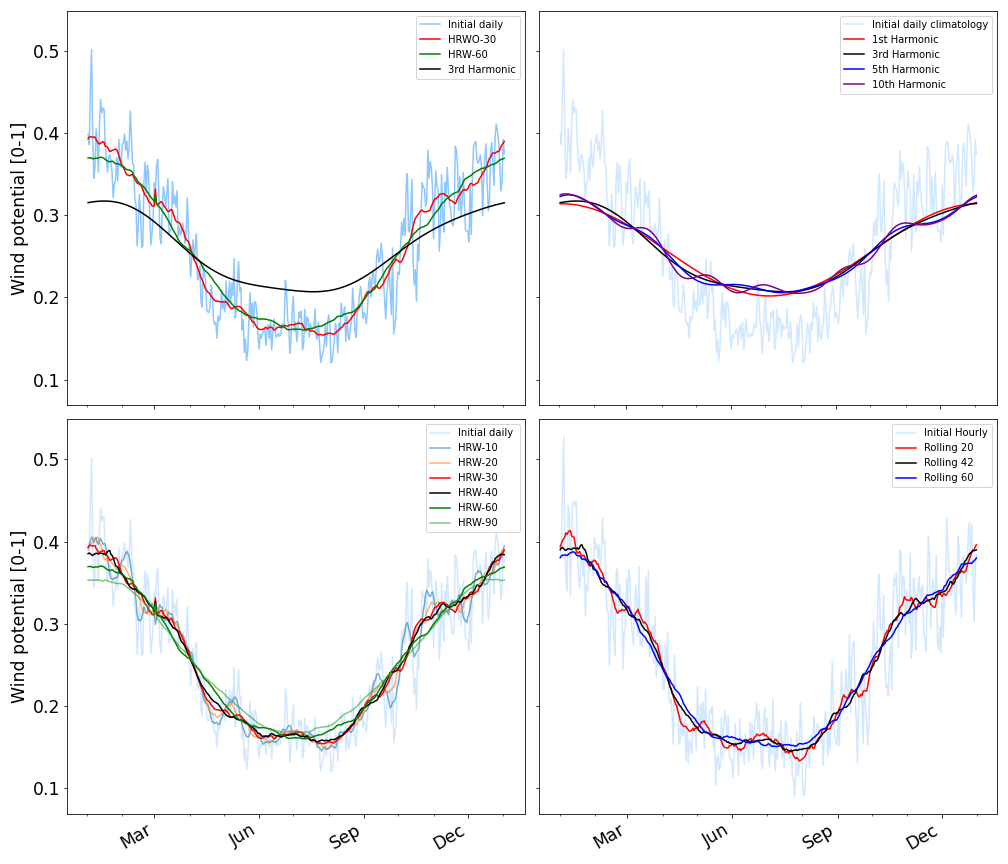
\includegraphics[width=0.9\textwidth]{Figures_SI/Fig_ClimatologyComparison_WON}
    \caption{
    Comparison of windows for the hourly rolling window (HRW) climate for wind during the period 1991-2020 for `NL01'. 
    In light blue the yearly generation potentials from 1991 to 2020 are shown. 
    The `initial' climate (grey, see main text for details) and various windows sizes (10,20,40,60,90,120 days) of the hourly rolling window climate (in purple, green, dark blue, yellow, black and orange, respectively) are shown.}
    \label{SIfig:clima_daily-harmonics_spv}
\end{figure}

\begin{figure}[t]
    \centering
    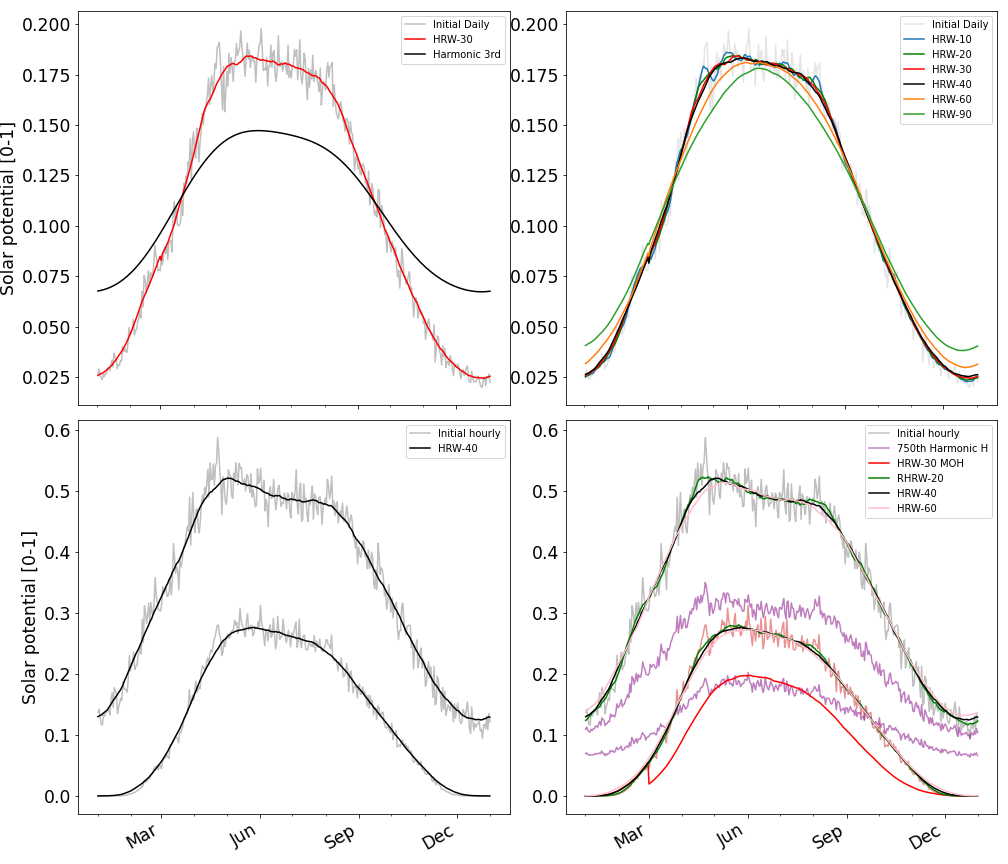
\includegraphics[width=0.9\textwidth]{Figures_SI/Fig_ClimatologyComparison_SPV}
    \caption{
    Comparison of windows for the hourly rolling window (HRW) climate for solar during the period 1991-2020 for `NL01'. 
    As shown in Figure~\ref{SIfig:clima_daily-harmonics_spv}, see legend for colours. }
    \label{SIfig:clima_daily-harmonics_won}
\end{figure}

\begin{figure}[ht!]
    \centering
    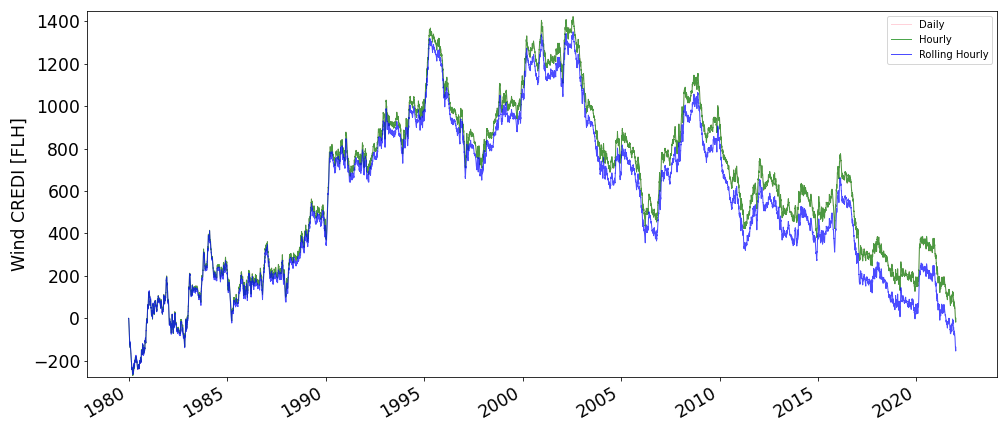
\includegraphics[width=0.9\textwidth]{Figures_SI/Fig_ClimComparison_WON}
    \caption{
    Comparison of the impact of a different climate definition on the resulting \credi{} for wind during the period 1991-2020 for `NL01'.}
    \label{SIfig:clima_impact}
\end{figure}

\clearpage






\subsection{Sensitivity of window size for Hourly Rolling Window climate definitions }\label{app:sense}
A comparison of windows for the hourly rolling window climate is shown in Figure~\ref{SIfig:clima_sense_solar} \& \ref{SIfig:clima_sense_zoom_solar} for solar and Figure~\ref{SIfig:clima_sense_wind} \& \ref{SIfig:clima_sense_zoom_wind} for wind. 

\begin{figure}[b]
    \centering
    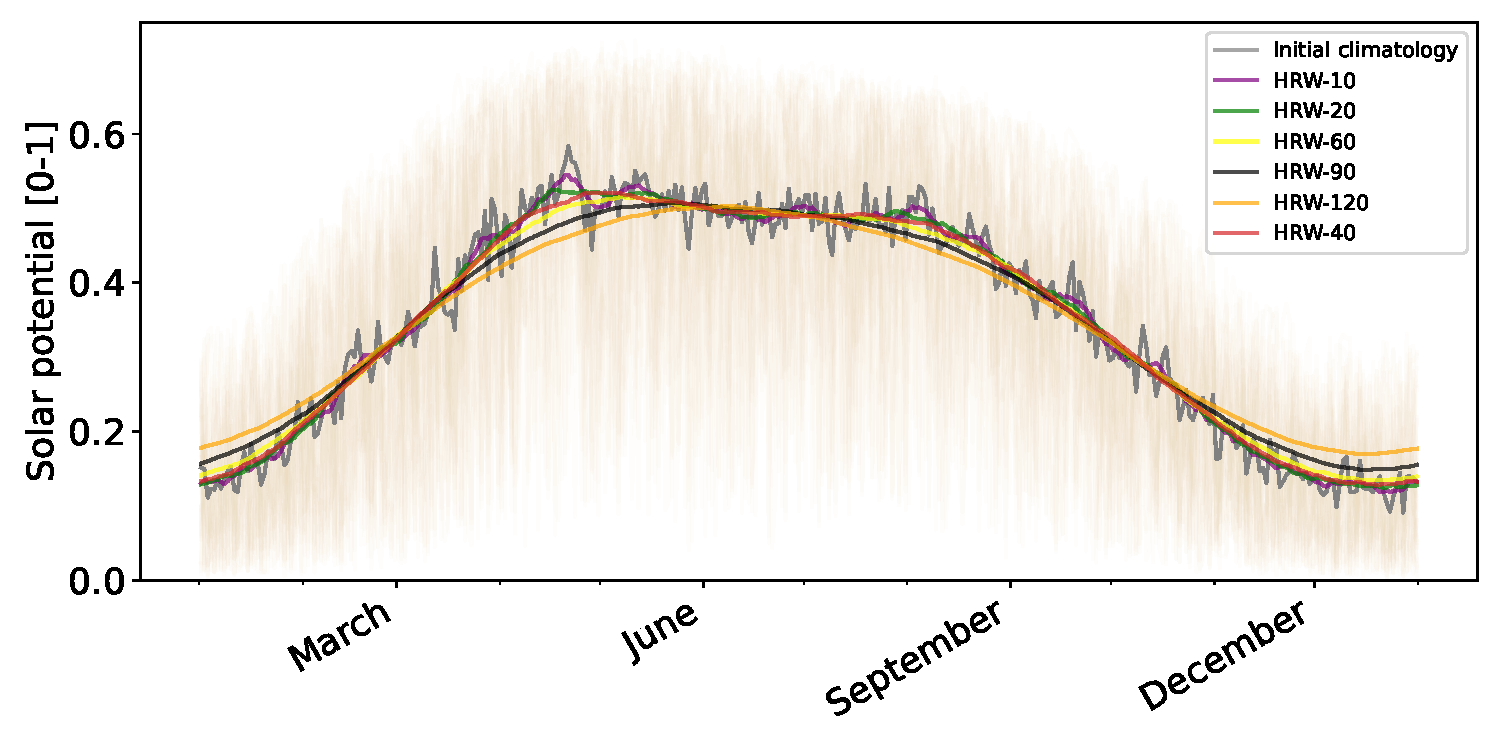
\includegraphics[width=\textwidth]{Figures_SI/Climatology_sensitivity_solar.pdf}
    \caption{Comparison of windows for the hourly rolling window (HRW) climate for solar during the period 1991-2020 for `NL01'. In light orange the yearly generation potentials from 1991 to 2020 are shown. The `initial' climate (grey, see main text for details) and various windows sizes (10,20,40,60,90,120 days) of the hourly rolling window climate (in purple, green, red, yellow, black and orange, respectively) are shown. For clarity only 13:00 for each day of the year is shown.}
    \label{SIfig:clima_sense_solar}
\end{figure}

% Solar
For solar potential the hourly rolling window climate for a 10 day window is not suited as variations are observed on daily to weekly timescales that have no physical reason to be a recurrent over the years (see Figure~\ref{SIfig:clima_sense_solar}). Similar to the climate for wind, these fluctuations observed at the 10 day window would not constitute as a good definition of a climate. On the other hand, very large windows like those using the 60, 90 or 120 window, are very smooth throughout the year, underestimating for instance the peak of maximum solar potential near the end of April/start of May (see Figure~\ref{SIfig:clima_sense_zoom_solar}) and severely over estimating the winter dip in solar potential (Figure~\ref{SIfig:clima_sense_solar}). Again, inline with what was found with wind this indicates an over-smoothing of the yearly cycle and thus using these windows within the hourly rolling window climate would thus not be a good indicator of likely weather. A window size in the range of 20-60 days is adequate in capturing the persistent weather fluctuations and the annual peak solar potential, without underestimating the annual cycle.


\begin{figure}[t]
    \centering
    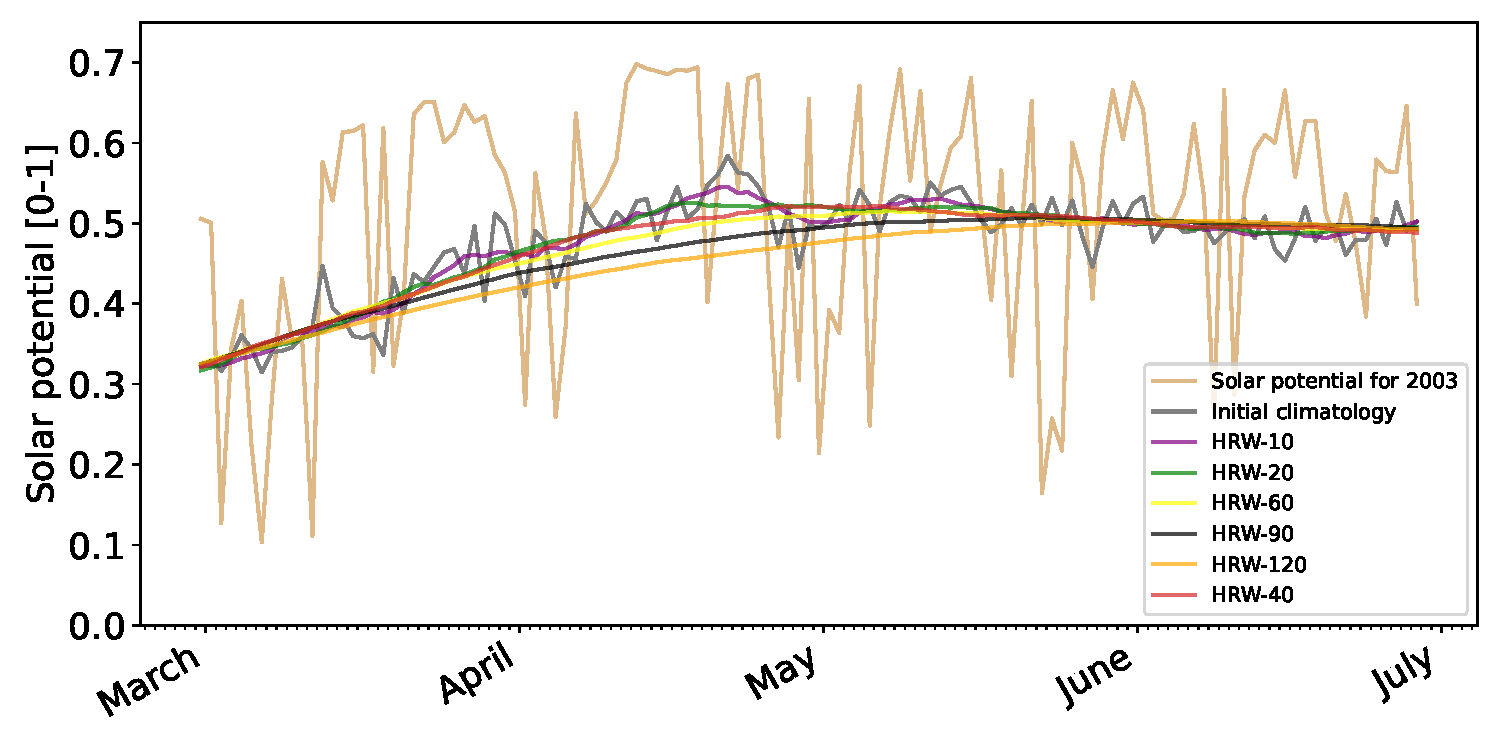
\includegraphics[width=\textwidth]{Figures_SI/Climatology_sensitivity_zoom_solar.pdf}
    \caption{Comparison of windows for the hourly rolling window climate for solar, as shown in Figure~\ref{SIfig:clima_sense_solar}, but specifically for the period from March to June 2003.}
    \label{SIfig:clima_sense_zoom_solar}
\end{figure}


% Wind
For wind potential the hourly rolling window climate for a 10 day window is not suited as variations are observed on daily to monthly timescales that have no physical reason to be a recurrent over the years (see Figure~\ref{SIfig:clima_sense_zoom_wind}). As a climate is defined as the statistically-mean weather conditions \emph{prevailing} in a region, the short-term nature of the fluctuations observed at the 10 day window would not constitute as a good definition of a climate as the climate fluctuates on short timescales. The same holds for the 20 day window, albeit to a lesser extent. On the other hand, very large windows like those using the 90 or 120 window, are very smooth throughout the year. For most of the mid-winter period their climate is well below the `initial' climate and during the summer above (see Figure~\ref{SIfig:clima_sense_wind}). This indicates an over-smoothing of the yearly cycle and thus using these windows within the hourly rolling window climate would thus not be a good indicator of likely weather. A window size in the range of 20-90 days is adequate in capturing the persistent weather fluctuations throughout the year, without underestimating the annual cycle.

\begin{figure}[hb]
    \centering
    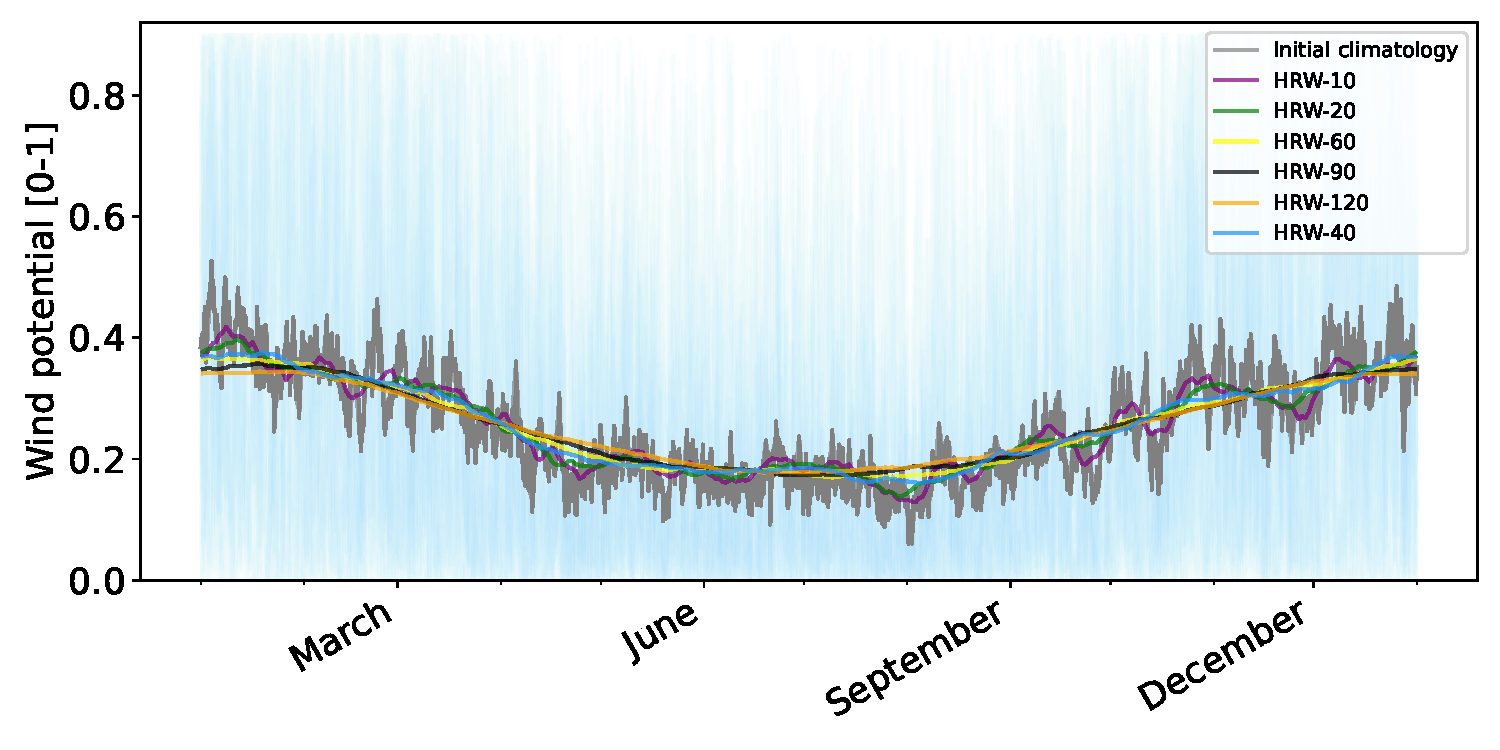
\includegraphics[width=\textwidth]{Figures_SI/Climatology_sensitivity_wind.pdf}
    \caption{Comparison of windows for the hourly rolling window (HRW) climate for wind during the period 1991-2020 for `NL01'. In light blue the yearly generation potentials from 1991 to 2020 are shown. The `initial' climate (grey, see main text for details) and various windows sizes (10,20,40,60,90,120 days) of the hourly rolling window climate (in purple, green, dark blue, yellow, black and orange, respectively) are shown.}
    \label{SIfig:clima_sense_wind}
\end{figure}

\begin{figure}[ht]
    \centering
    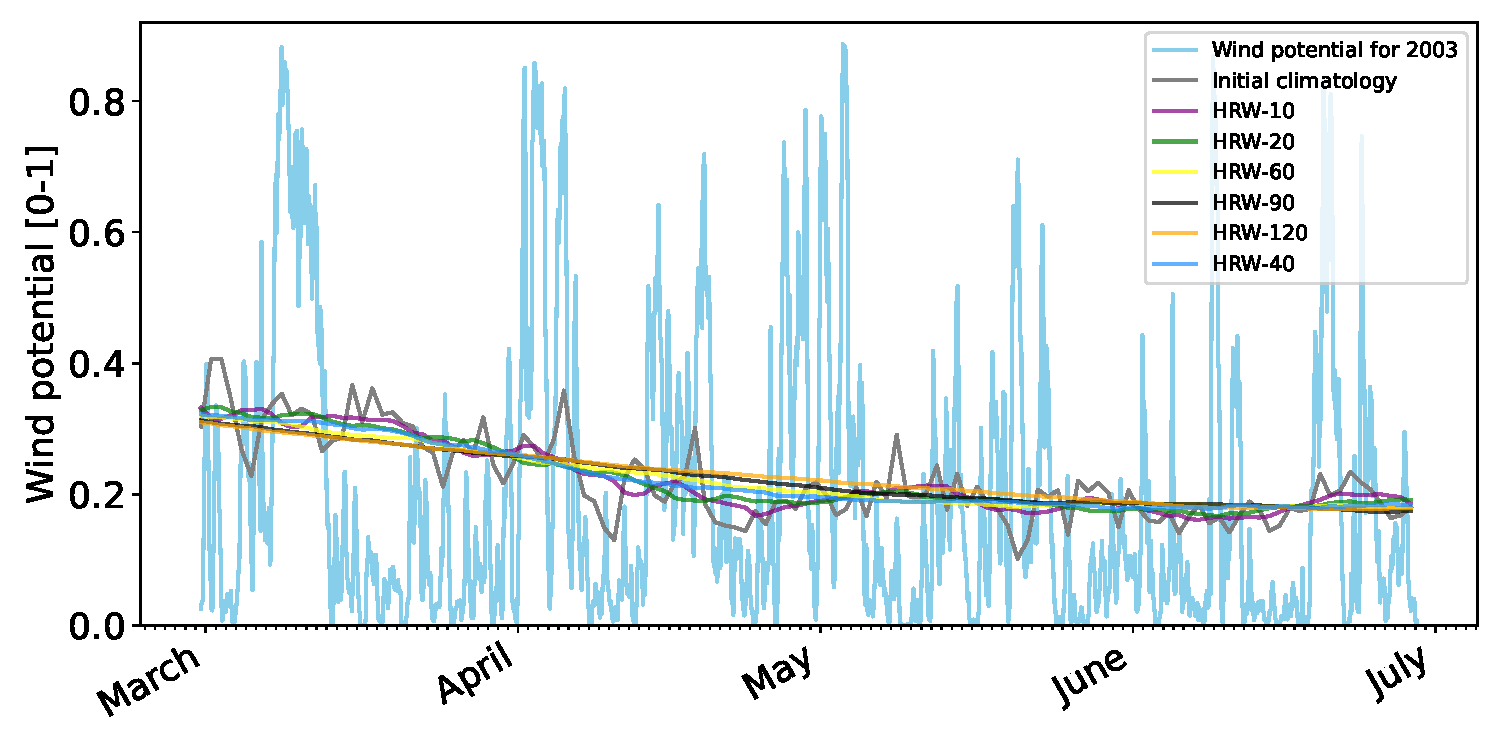
\includegraphics[width=\textwidth]{Figures_SI/Climatology_sensitivity_zoom_wind.pdf}
    \caption{Comparison of windows for the hourly rolling window climate for wind for `NL01', as shown in Figure~\ref{SIfig:clima_sense_wind}, but specifically for the period from March to June 2003.}
    \label{SIfig:clima_sense_zoom_wind}
\end{figure}



%%%%%%%%%%%%%%%%%%%%%%%%%%%%%%%%%%%%%%%%%%%%%%%%%%
%%%%		~~~~ Comparison of analysis start point ~~~~

% \clearpage
\section{Annual start date analysis for \credi}\label{app:startdate}
Section 4 in the main text describes the application of the \credi{} at different timescales. 
Here we show how the hourly distribution of \credi{} changes over a year if a different starting point is used (Figures~\ref{SIfig:startdate_solar} \& \ref{SIfig:startdate_wind}). 
In line with the main text four exemplary storylines are shown, namely 1996 (red), 1998 (green), 2003 (purple) and 2016 (black).

% Quick observation
From Figure~\ref{SIfig:startdate_wind}, the impact of choosing a different starting point becomes very clear.  
For the storylines shown you can see that they change from one of the highest, to on of the lowest depending on the start point. 
To a lesser degree, the same holds for the solar resource shown in  Figure~\ref{SIfig:startdate_solar}.

\begin{figure}[t]
\centering
\begin{subfigure}[t]{0.32\linewidth}
    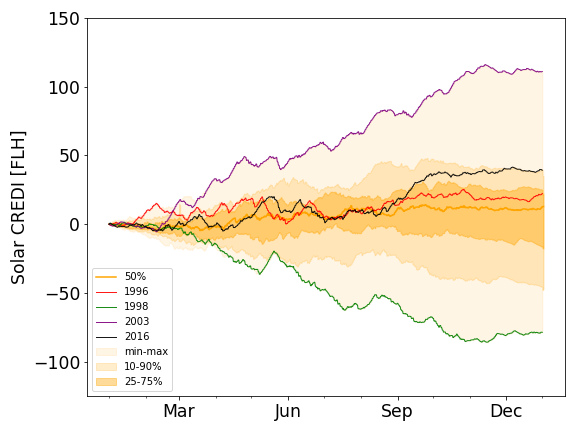
\includegraphics[width=\linewidth]{Figures_SI/Fig_CUMSUM_YearStart_SPV_January}
    \caption{January }
\end{subfigure}
\begin{subfigure}[t]{0.32\linewidth}
    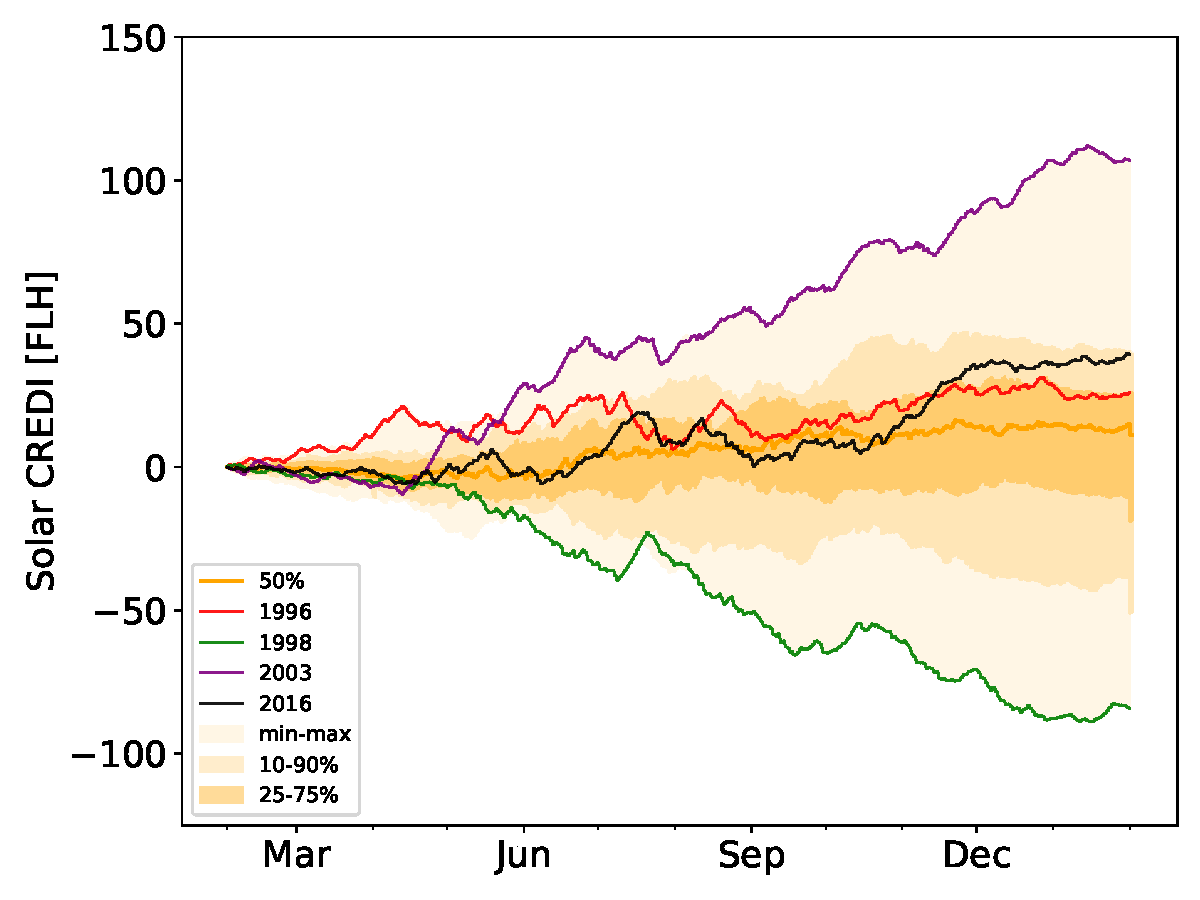
\includegraphics[width=\linewidth]{Figures_SI/Fig_CUMSUM_YearStart_SPV_February}
    \caption{Febuary }
\end{subfigure}
\begin{subfigure}[t]{0.32\linewidth}
    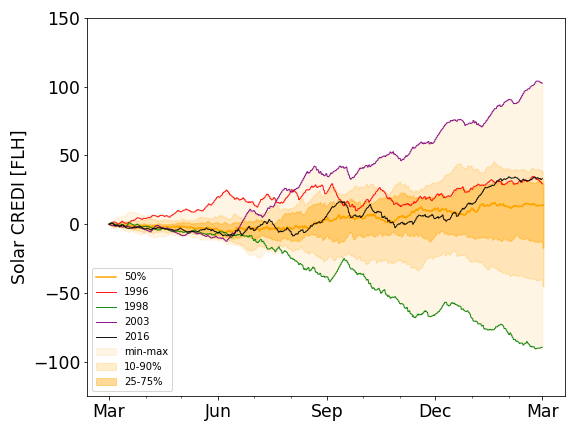
\includegraphics[width=\linewidth]{Figures_SI/Fig_CUMSUM_YearStart_SPV_March}
    \caption{March }
\end{subfigure}
\begin{subfigure}[t]{0.32\linewidth}
    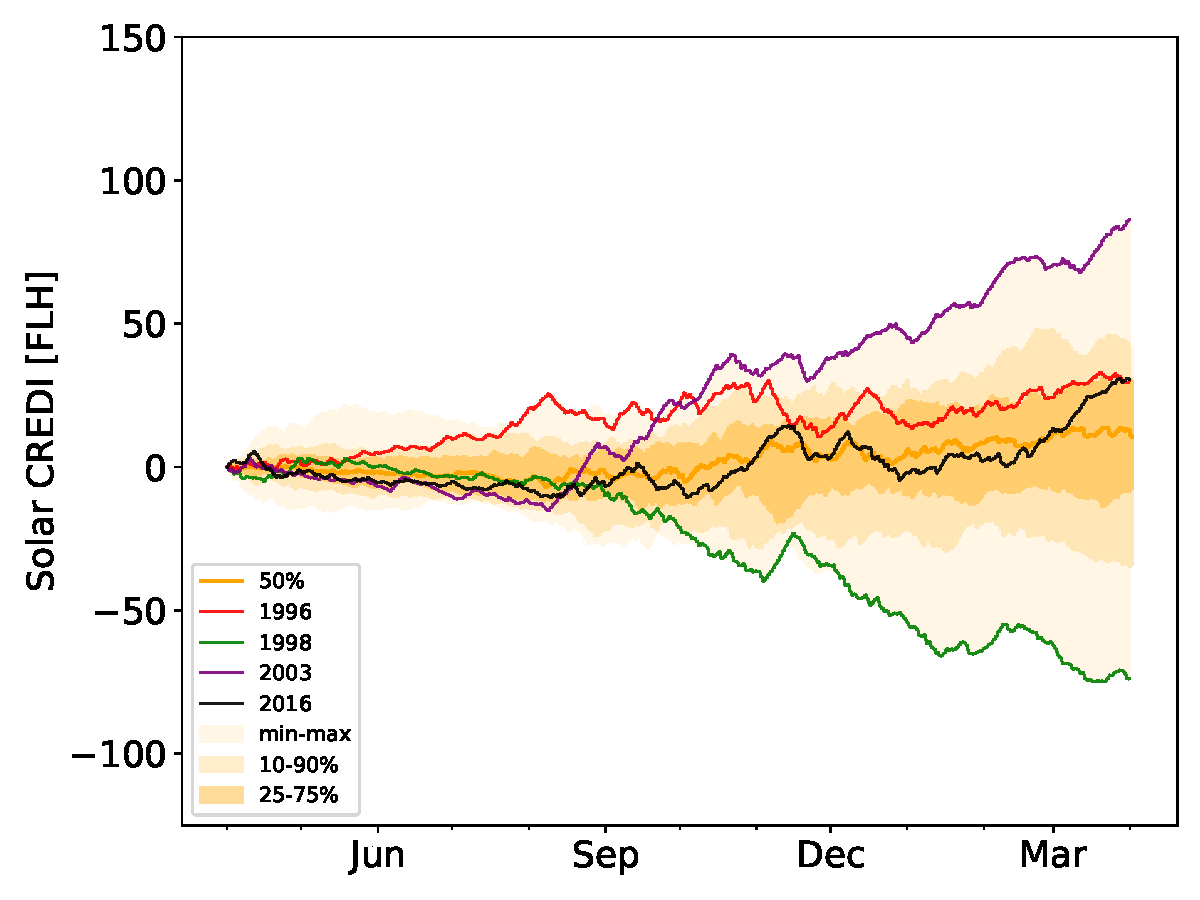
\includegraphics[width=\linewidth]{Figures_SI/Fig_CUMSUM_YearStart_SPV_April}
    \caption{April }
\end{subfigure}
\begin{subfigure}[t]{0.32\linewidth}
    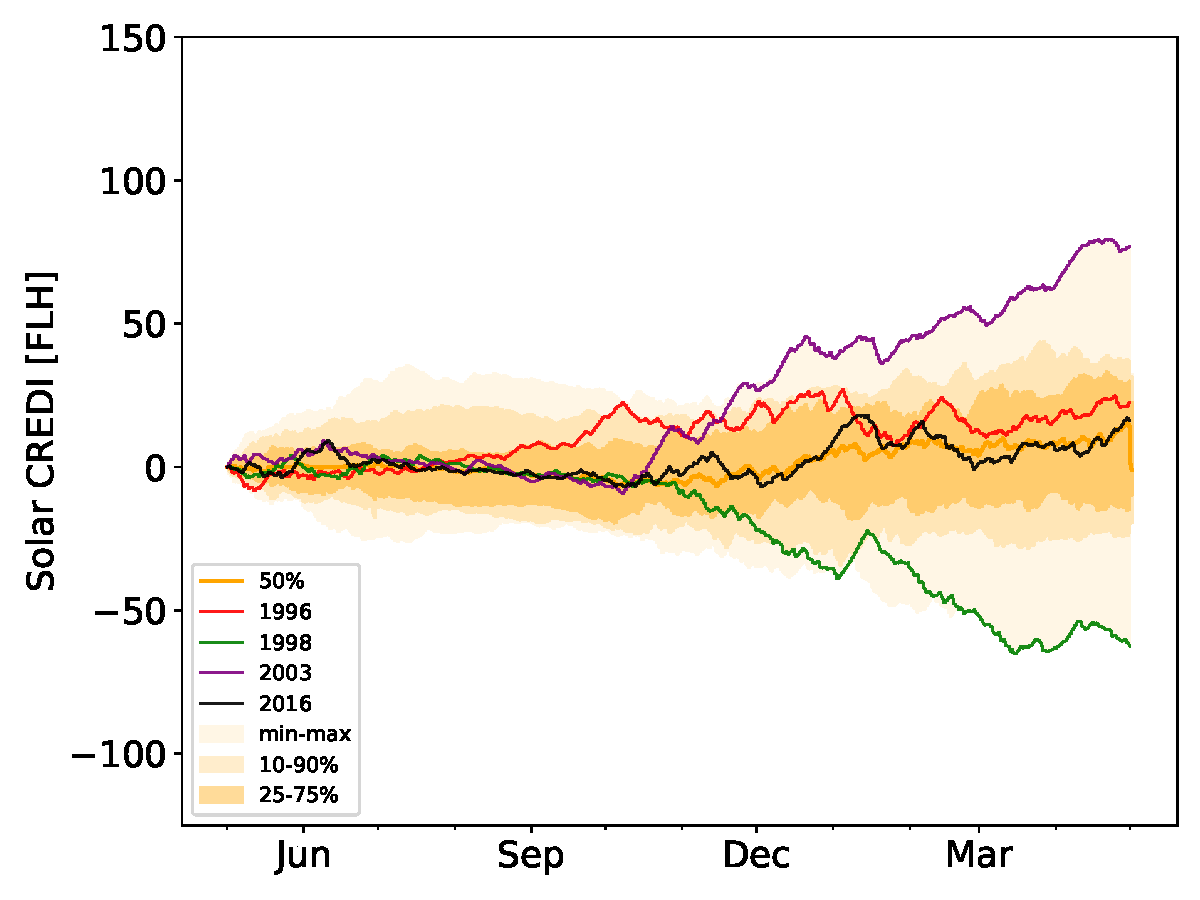
\includegraphics[width=\linewidth]{Figures_SI/Fig_CUMSUM_YearStart_SPV_May}
    \caption{May }
\end{subfigure}
\begin{subfigure}[t]{0.32\linewidth}
    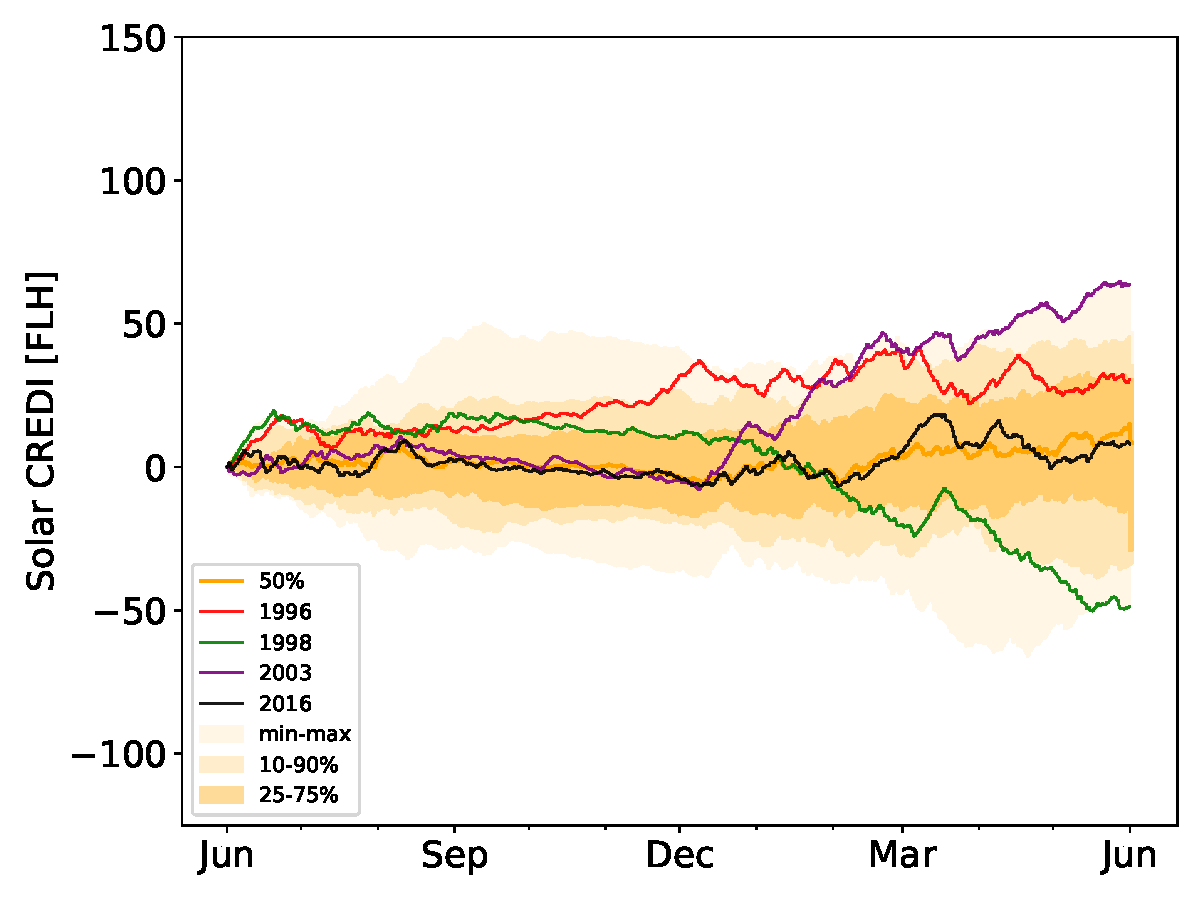
\includegraphics[width=\linewidth]{Figures_SI/Fig_CUMSUM_YearStart_SPV_June}
    \caption{June }
\end{subfigure}
\begin{subfigure}[t]{0.32\linewidth}
    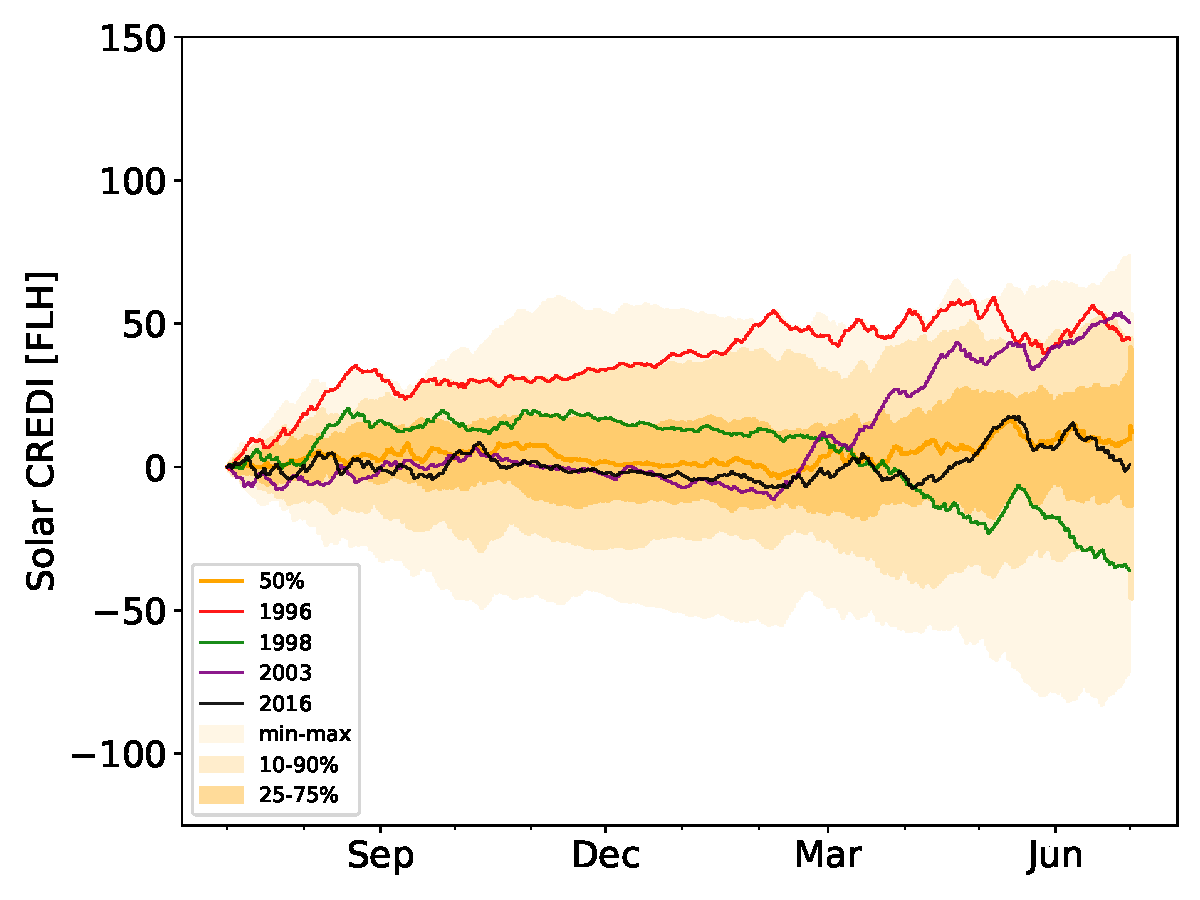
\includegraphics[width=\linewidth]{Figures_SI/Fig_CUMSUM_YearStart_SPV_July}
    \caption{July }
\end{subfigure}
\begin{subfigure}[t]{0.32\linewidth}
    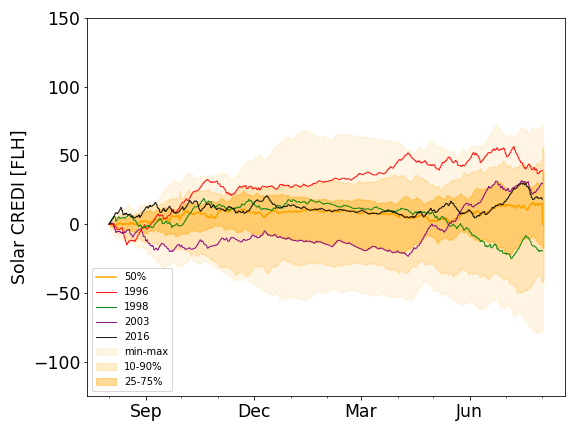
\includegraphics[width=\linewidth]{Figures_SI/Fig_CUMSUM_YearStart_SPV_August}
    \caption{August }
\end{subfigure}
\begin{subfigure}[t]{0.32\linewidth}
    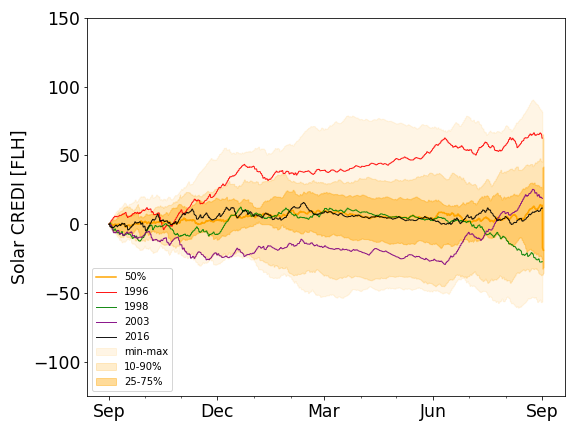
\includegraphics[width=\linewidth]{Figures_SI/Fig_CUMSUM_YearStart_SPV_September}
    \caption{September }
\end{subfigure}
\begin{subfigure}[t]{0.32\linewidth}
    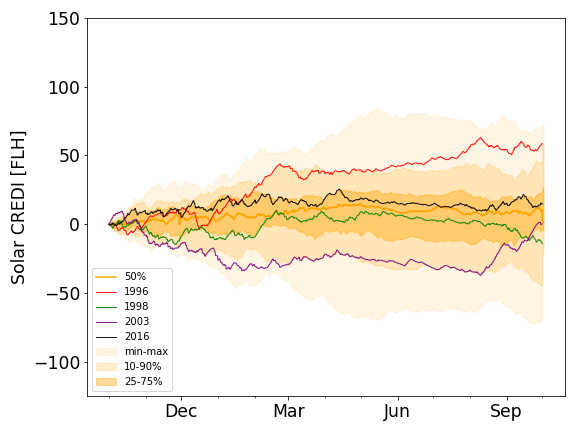
\includegraphics[width=\linewidth]{Figures_SI/Fig_CUMSUM_YearStart_SPV_October}
    \caption{October }
\end{subfigure}
\begin{subfigure}[t]{0.32\linewidth}
    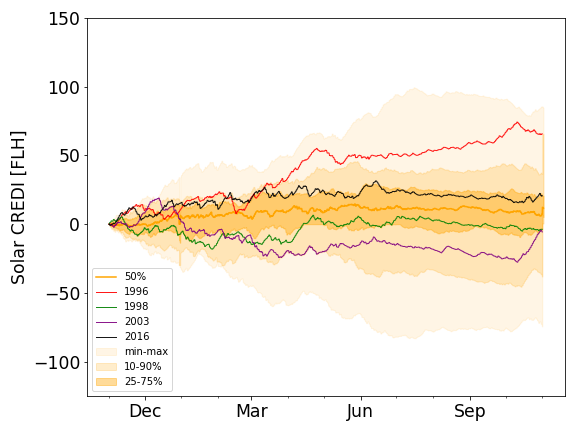
\includegraphics[width=\linewidth]{Figures_SI/Fig_CUMSUM_YearStart_SPV_November}
    \caption{November}
\end{subfigure}
\begin{subfigure}[t]{0.32\linewidth}
    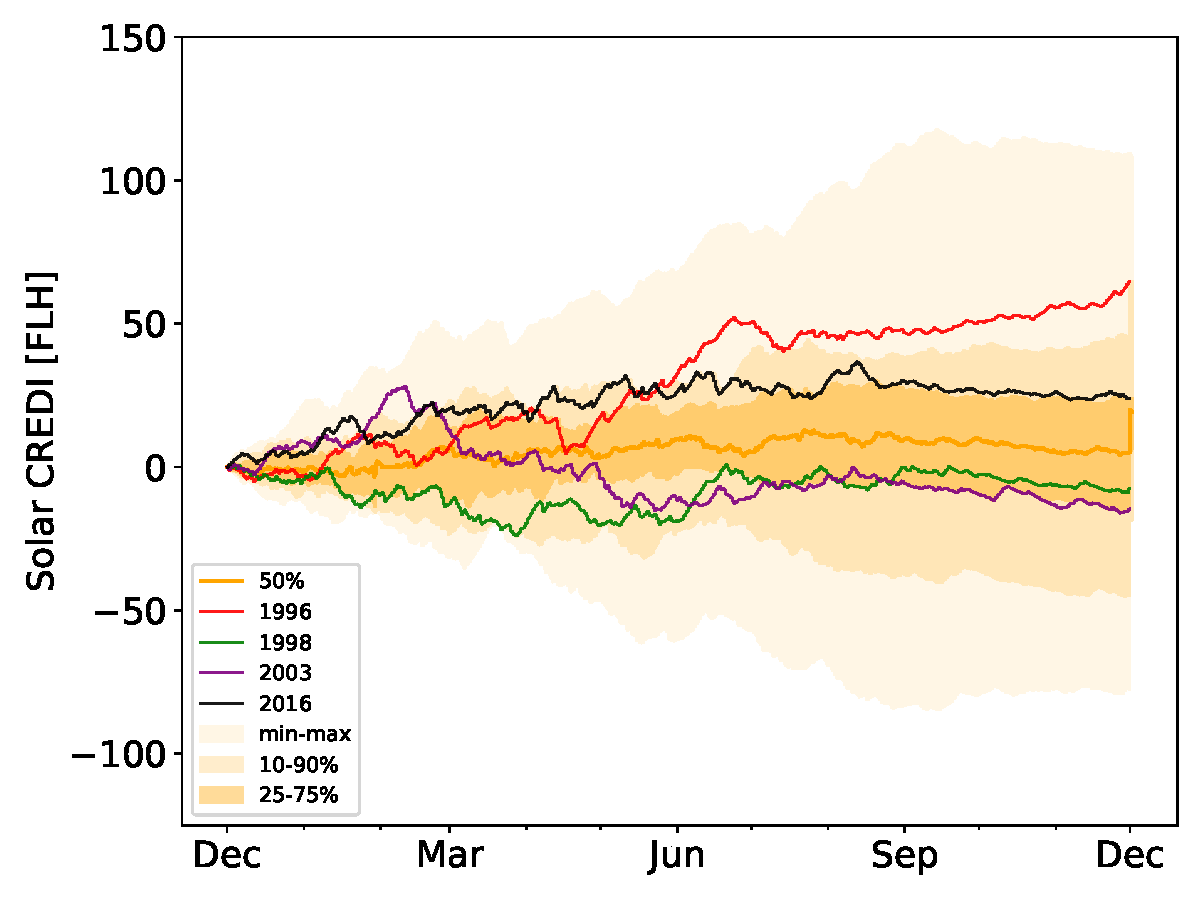
\includegraphics[width=\linewidth]{Figures_SI/Fig_CUMSUM_YearStart_SPV_December}
    \caption{December }
\end{subfigure}
\caption{
    Comparison of the distribution of the \sdi{} with different the monthly starting points of the annual period. 
    The distribution is shown with the 50\ts{th} percentile (orange line), the 25-75, 10-90 percentile and min-max range (shaded orange, see legend) for each hour of the year for the years 1991-2020 in the `NL01' region. 
    Four exemplary storylines are shown, namely 1996 (red), 1998 (green), 2003 (purple) and 2016 (black), see main text for details and analysis.}
\label{SIfig:startdate_solar}
\end{figure}



\begin{figure}[b]
\centering
\begin{subfigure}[t]{0.32\linewidth}
    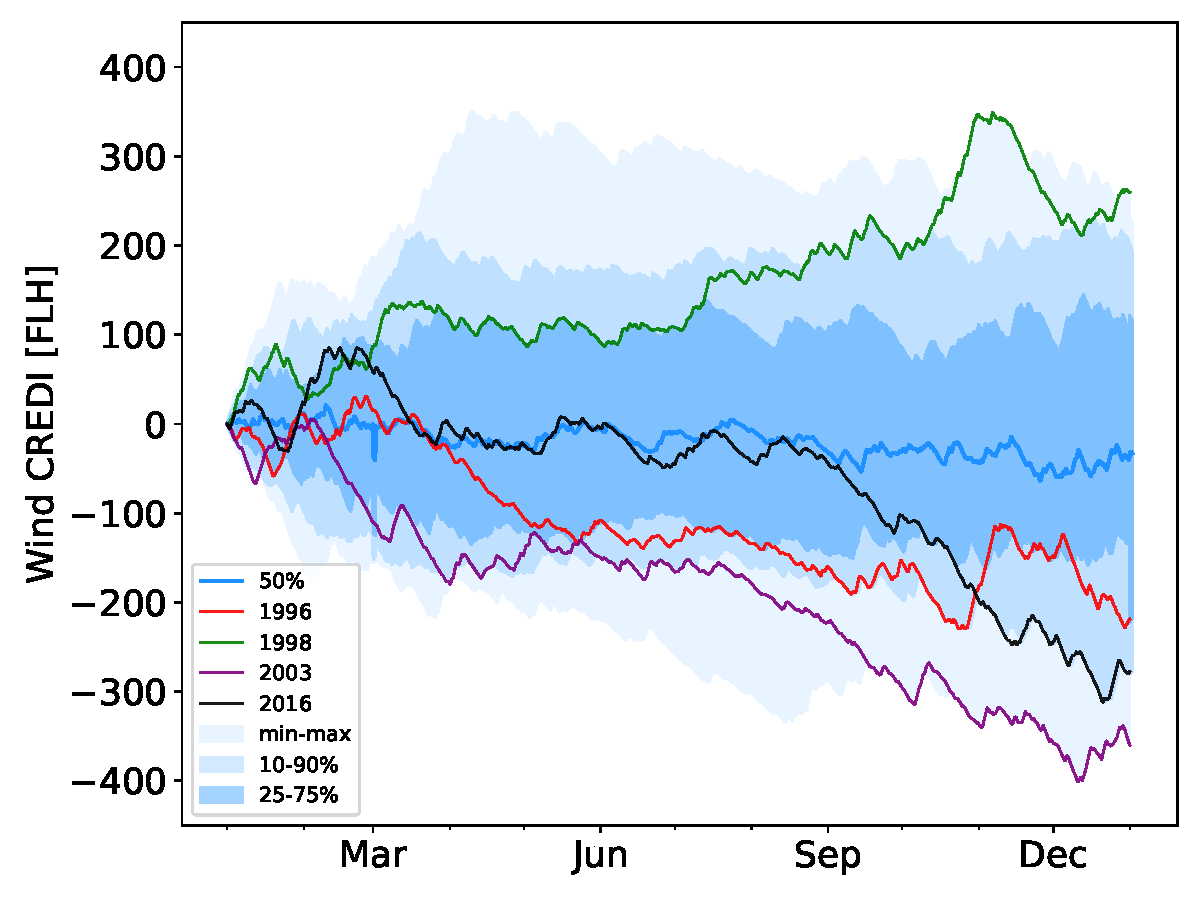
\includegraphics[width=\linewidth]{Figures_SI/Fig_CUMSUM_YearStart_January}
    \caption{January }
\end{subfigure}
\begin{subfigure}[t]{0.32\linewidth}
    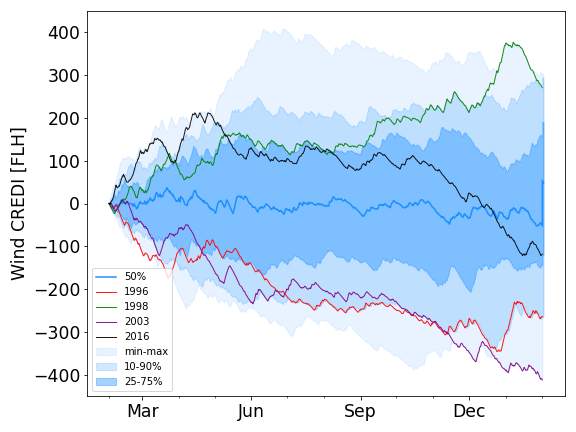
\includegraphics[width=\linewidth]{Figures_SI/Fig_CUMSUM_YearStart_February}
    \caption{Febuary }
\end{subfigure}
\begin{subfigure}[t]{0.32\linewidth}
    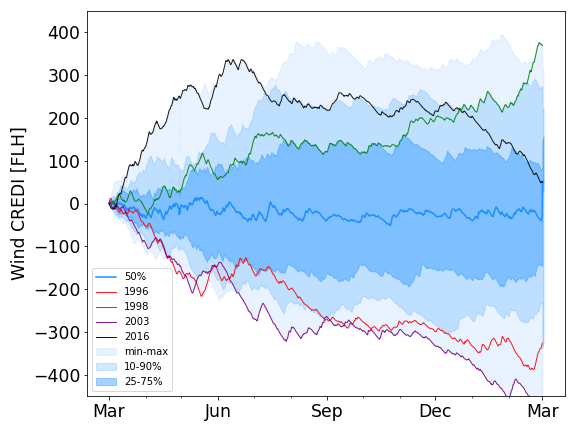
\includegraphics[width=\linewidth]{Figures_SI/Fig_CUMSUM_YearStart_March}
    \caption{March }
\end{subfigure}
\begin{subfigure}[t]{0.32\linewidth}
    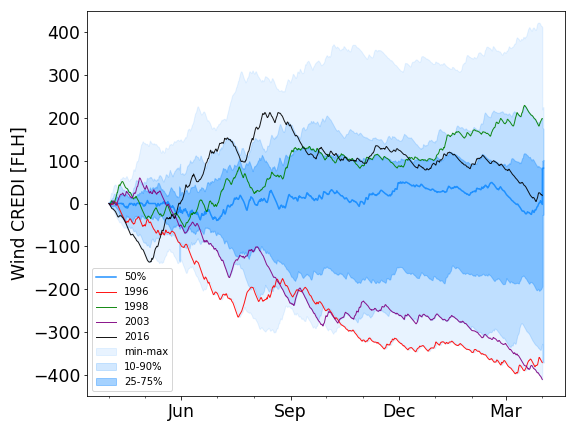
\includegraphics[width=\linewidth]{Figures_SI/Fig_CUMSUM_YearStart_April}
    \caption{April }
\end{subfigure}
\begin{subfigure}[t]{0.32\linewidth}
    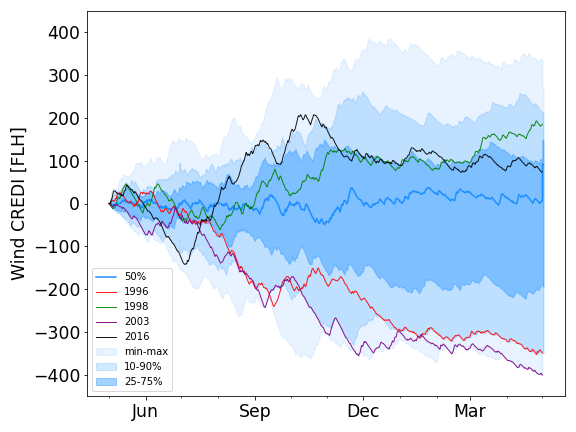
\includegraphics[width=\linewidth]{Figures_SI/Fig_CUMSUM_YearStart_May}
    \caption{May }
\end{subfigure}
\begin{subfigure}[t]{0.32\linewidth}
    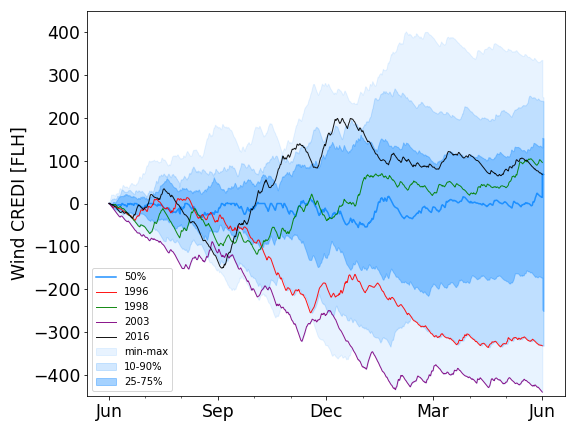
\includegraphics[width=\linewidth]{Figures_SI/Fig_CUMSUM_YearStart_June}
    \caption{June }
\end{subfigure}
\begin{subfigure}[t]{0.32\linewidth}
    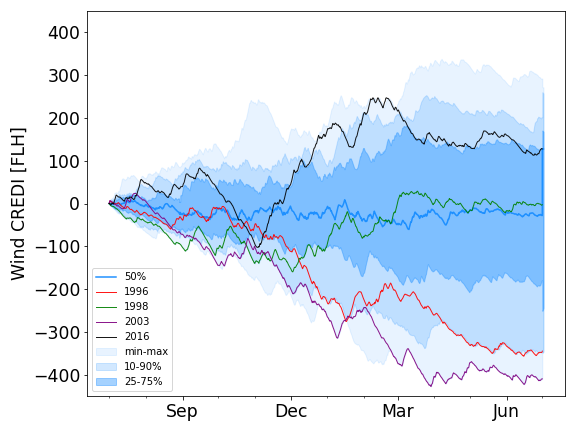
\includegraphics[width=\linewidth]{Figures_SI/Fig_CUMSUM_YearStart_July}
    \caption{July }
\end{subfigure}
\begin{subfigure}[t]{0.32\linewidth}
    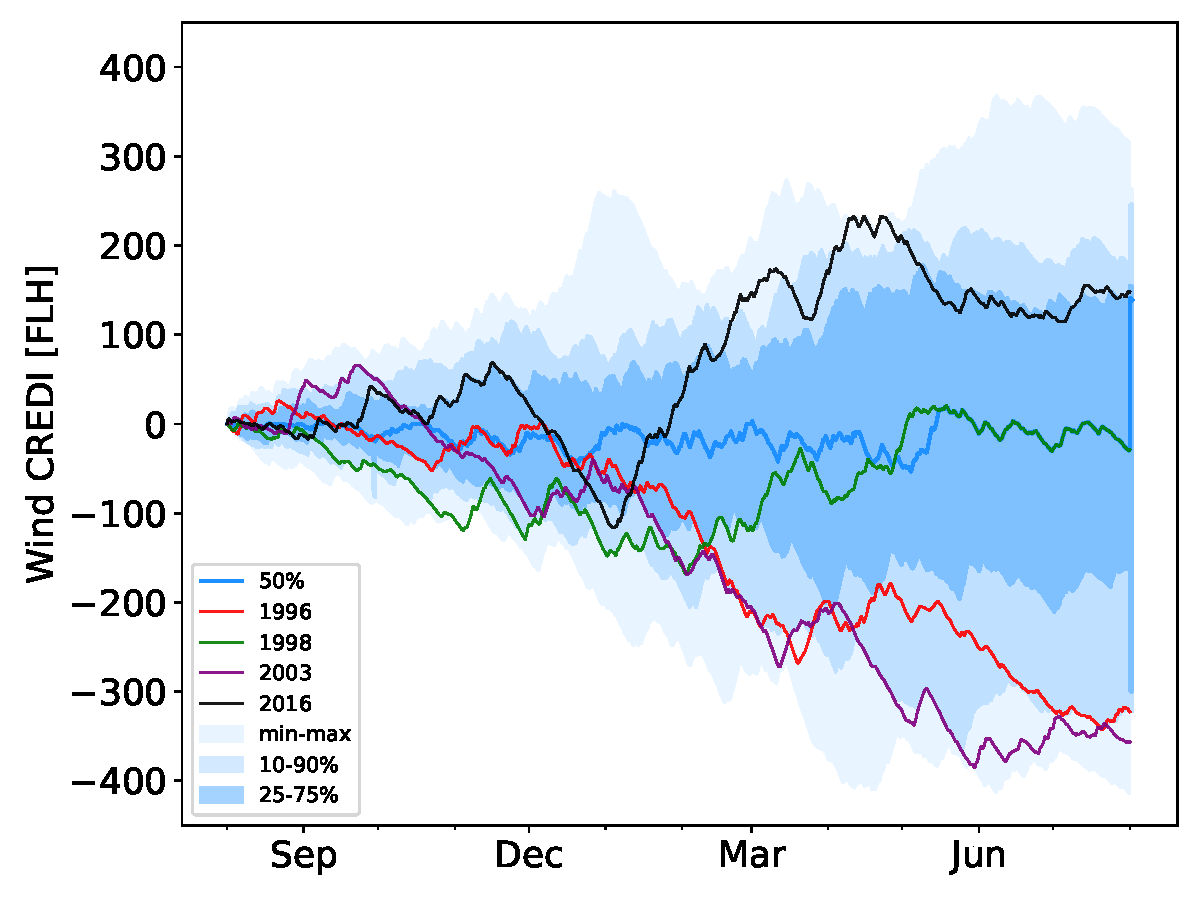
\includegraphics[width=\linewidth]{Figures_SI/Fig_CUMSUM_YearStart_August}
    \caption{August }
\end{subfigure}
\begin{subfigure}[t]{0.32\linewidth}
    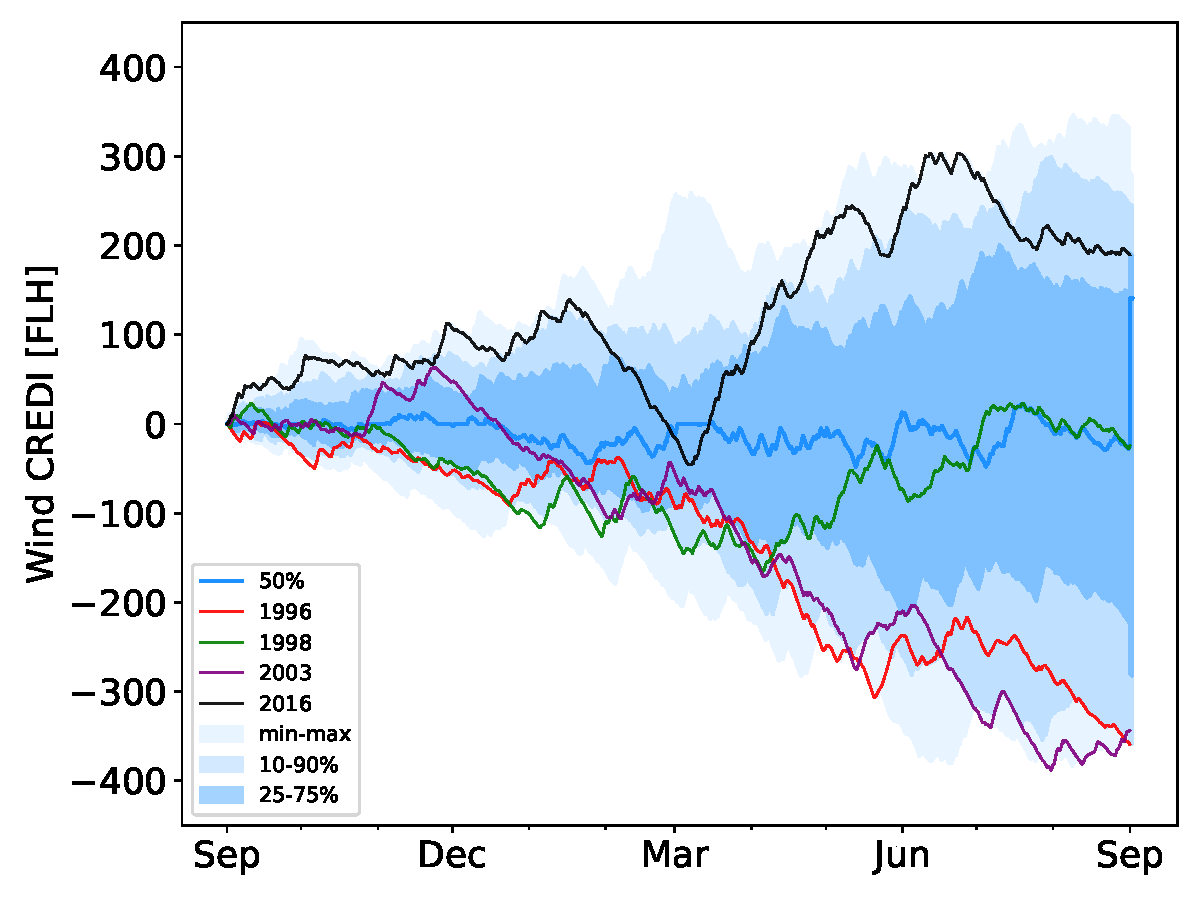
\includegraphics[width=\linewidth]{Figures_SI/Fig_CUMSUM_YearStart_September}
    \caption{September }
\end{subfigure}
\begin{subfigure}[t]{0.32\linewidth}
    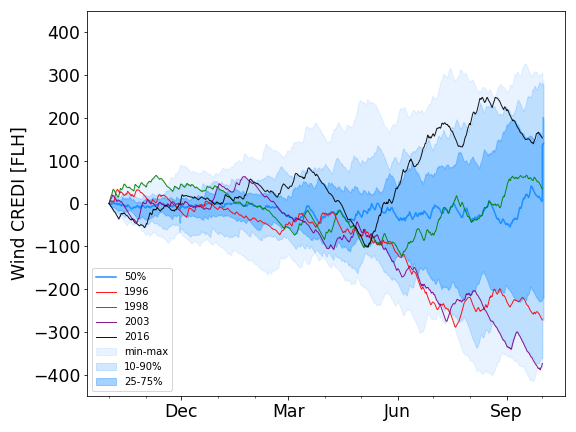
\includegraphics[width=\linewidth]{Figures_SI/Fig_CUMSUM_YearStart_October}
    \caption{October }
\end{subfigure}
\begin{subfigure}[t]{0.32\linewidth}
    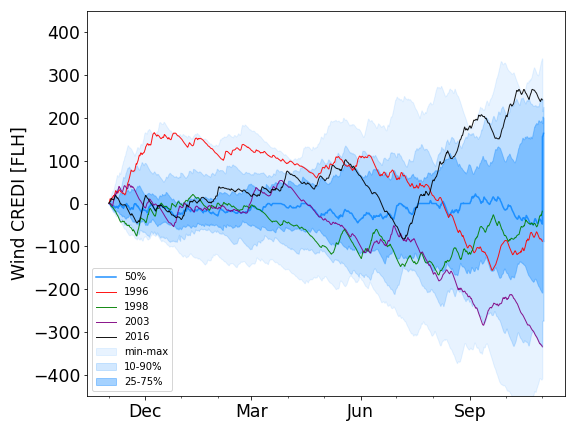
\includegraphics[width=\linewidth]{Figures_SI/Fig_CUMSUM_YearStart_November}
    \caption{November}
\end{subfigure}
\begin{subfigure}[t]{0.32\linewidth}
    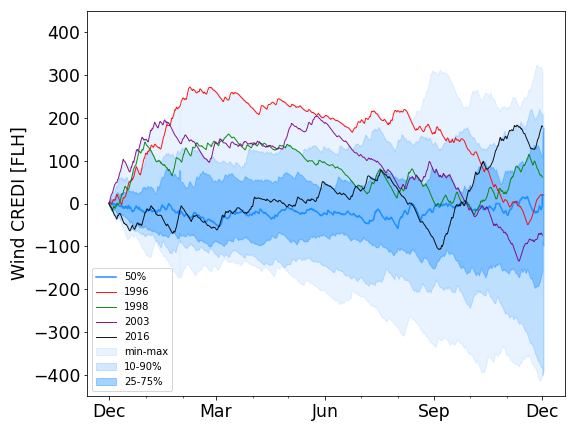
\includegraphics[width=\linewidth]{Figures_SI/Fig_CUMSUM_YearStart_December}
    \caption{December }
\end{subfigure}
\caption{
    Comparison of the distribution of the \wdi{} with different the monthly starting points of the annual period. 
    The distribution is shown with the 50\ts{th} percentile (blue line), the 25-75, 10-90 percentile and min-max range (shaded blue, see legend) for each hour of the year for the years 1991-2020 in the `NL01' region. 
    Four exemplary storylines are shown, namely 1996 (red), 1998 (green), 2003 (purple) and 2016 (black), see main text for details and analysis.}
\label{SIfig:startdate_wind}
\end{figure}




%%%%%%%%%%%%%%%%%%%%%%%%%%%%%%%%%%%%%%%%%%%%%%%%%%
%%%%		~~~~ Seasonal behaviour of CREDI ~~~~

\clearpage
\section{Additional seasonal analysis figures of \credi}\label{app:seasonal}
Section 4.3 in the main text shows the seasonal variability in \credi.
Here we provide some additional figures representing a different season for either {\sc wind} or \sdi{} (Figures~\ref{SIfig:analysis_season-summer_wind}-\ref{SIfig:analysis_season-winter_solar}). 

\begin{figure}[h]
    \centering
    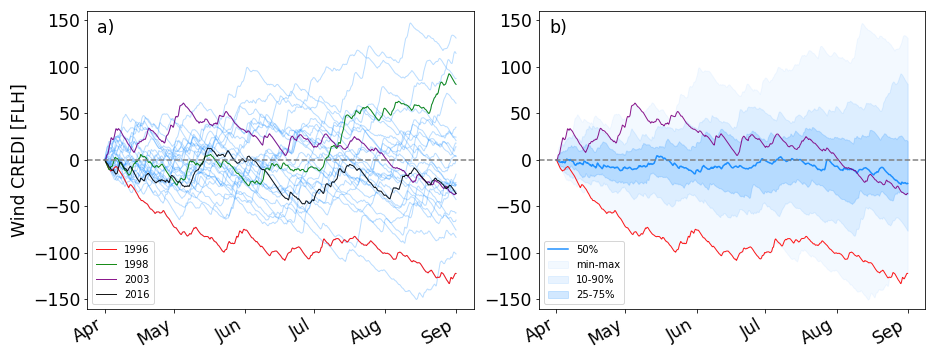
\includegraphics[width=\textwidth]{Figures_SI/WindCREDI_seasonal-summer}
    \caption{
    Hourly summer \wdi{} throughout the season over the period 1991-2020 for `NL01'.
    Figure a) shows the specific progression of \wdi{} for each summer season (blue lines).
    In addition, four example storylines are represented, namely 1996 (red), 1998(green), 2003(purple) and 2016 (black), see main text for details and analysis.
    Figure b) shows two storylines (1996, 2003) and the hourly distribution of the \wdi{}, namely the 50\ts{th} percentile (blue line), the 25-75, 10-90 percentile, and min-max range (shaded blue, see legend). 
    }
    \label{SIfig:analysis_season-summer_wind}
\end{figure}
\begin{figure}[b!]
    \centering
    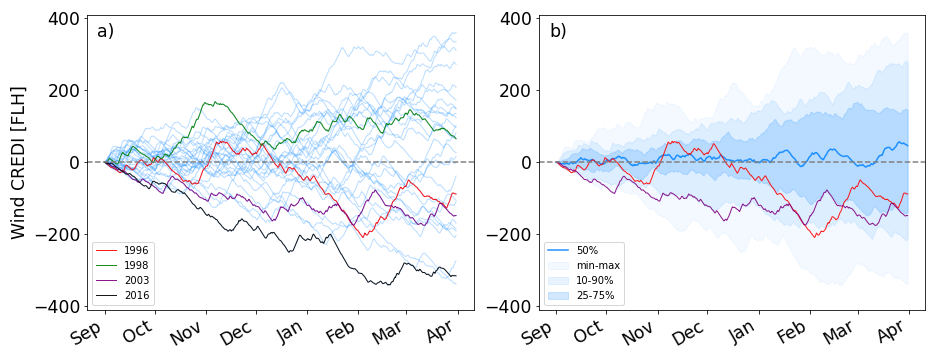
\includegraphics[width=\textwidth]{Figures_SI/WindCREDI_seasonal-winter}
    \caption{
    Hourly winter \wdi{} throughout the season over the period 1991-2020 for `NL01'.
    As shown in Figure~\ref{SIfig:analysis_season-summer_wind}.
    }
    \label{SIfig:analysis_season-winter_wind}
\end{figure}

\begin{figure}[ht!]
    \centering
    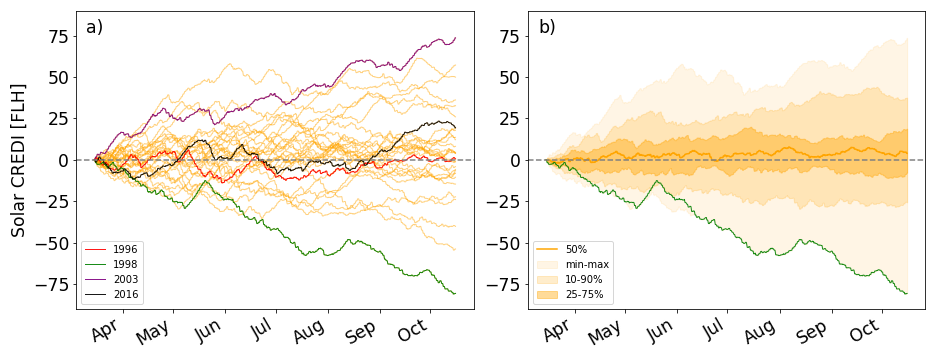
\includegraphics[width=\textwidth]{Figures_SI/SolarCREDI_seasonal-summer}
    \caption{
    Hourly summer \sdi{} throughout the season over the period 1991-2020 for `NL01'.
    Figure a) shows the specific progression of \sdi{} for each summer season (orange lines).
    In addition, four example storylines are represented, namely 1996 (red), 1998(green), 2003(purple) and 2016 (black), see main text for details and analysis.
    Figure b) shows two storylines (1996, 2003) and the hourly distribution of the \sdi{}, namely the 50\ts{th} percentile (orange line), the 25-75, 10-90 percentile, and min-max range (shaded orange, see legend). 
    }
    \label{SIfig:analysis_season-summer_solar}
\end{figure}
\begin{figure}[h!]
    \centering
    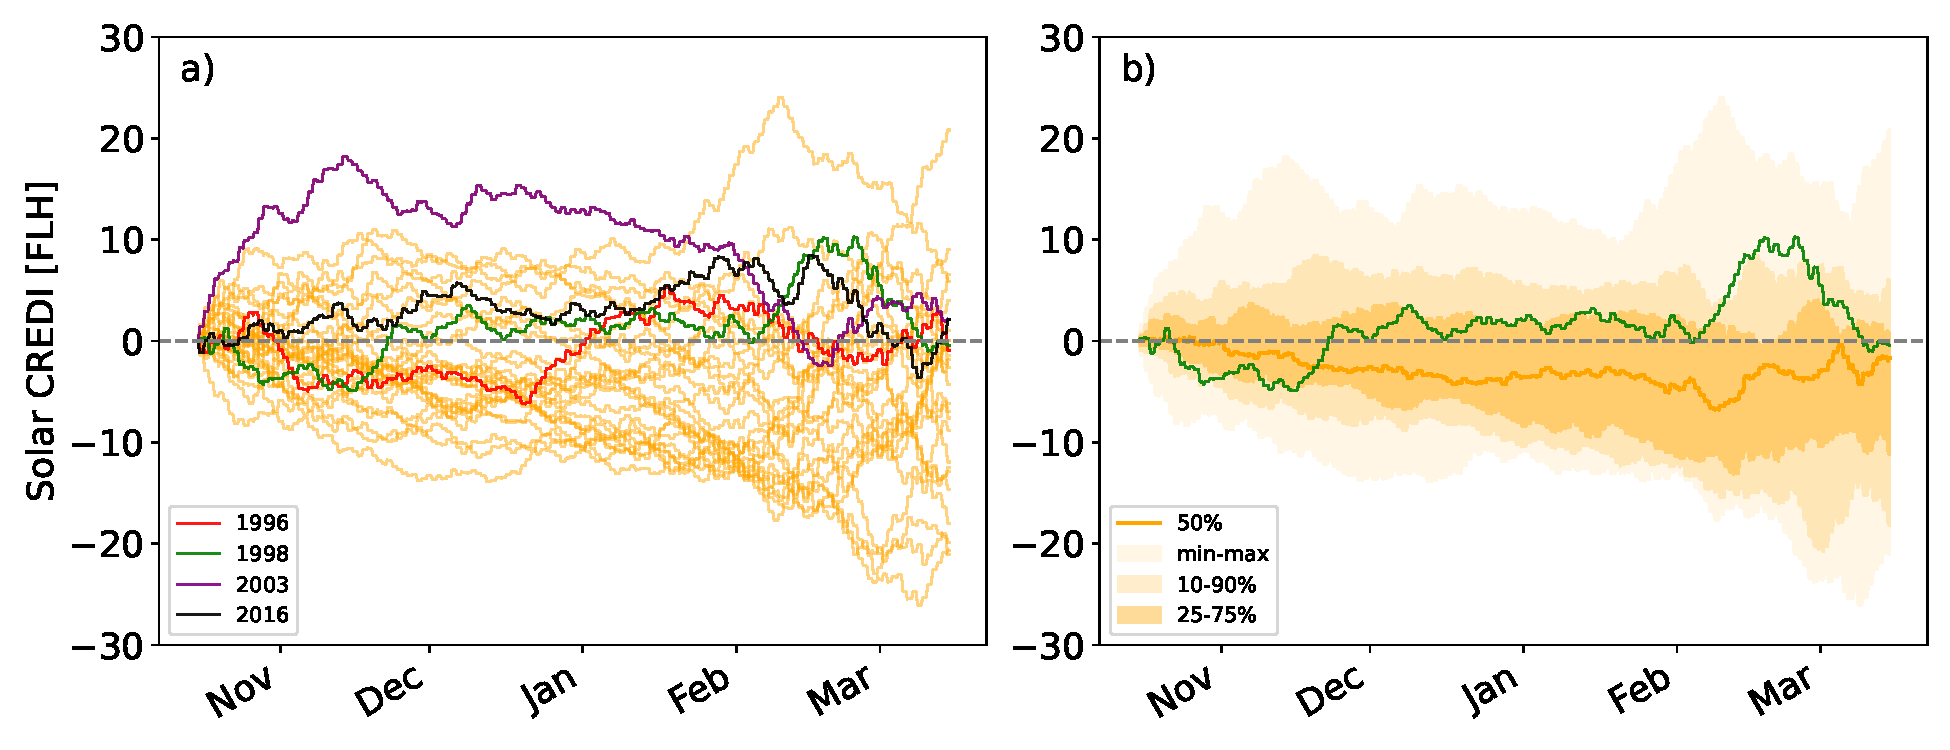
\includegraphics[width=\textwidth]{Figures_SI/SolarCREDI_seasonal-winter}
    \caption{
    Hourly winter \sdi{} throughout the season over the period 1991-2020 for `NL01'.
    As shown in Figure~\ref{SIfig:analysis_season-summer_solar}.
    }
    \label{SIfig:analysis_season-winter_solar}
\end{figure}


%%%%%%%%%%%%%%%%%%%%%%%%%%%%%%%%%%%%%%%%%%%%%%%%%%
%%%%		~~~~ Short-term behaviour of CREDI ~~~~

\clearpage
\section{Additional short-term analysis figures of \credi}\label{app:shortterm}
Section 4.4 in the main text shows an example of the short-term \credi{} event selection.
Here we provide some additional figures related to the event selection and the observed behaviour.  
Figure~\ref{SIfig:analysis_short-term-winter_wind_behaviour} shows the wind distribution of the generation potential during the analysis period and for the selected events.

%% short-term behaviour
\begin{figure}[h]
        \centering
        \includegraphics[width=\textwidth]{Figures_SI/WindCREDI_shortterm_behaviour}
        % \includegraphics[width=\textwidth]{Mainmatter/CP2/Figures/WindCREDI_shortterm_behaviour}
        \caption{
                Hourly winter \wdi{} per 8-days for all events with less then 5 days overlapping in the period May 1991 to April 2021 for `NL01'. 
                The storylines show the analysis years 1996 (red, 4x), 1998 (green, 1x), 2003 (purple, 1x) and 2016 (black, 3x). 
                Figure a) shows the specific progression of \wdi{} for each summer season (blue lines). 
                To highlight the behaviour during an event, Figure b) shows the hourly distribution of the wind generation potential, namely the 50\ts{th} percentile (blue line), the 25-75, 10-90 percentile, and min-max range (shaded blue, see legend).
        }
        \label{SIfig:analysis_short-term-winter_wind_behaviour}
\end{figure}

%% short-term histogram
\begin{figure}[h]
        \centering
        \includegraphics[width=\textwidth]{Figures_SI/CREDI_shortterm_histogram}
        % \includegraphics[width=\textwidth]{Mainmatter/CP2/Figures/CREDI_shortterm_histogram}
        \caption{
                Histogram of the \sdi{} (Figure a) and \wdi{} (Figure b) at 8-days for all events with less then 5 days overlapping in the period May 1991 to April 2021 for `NL01'. 
        }
        \label{SIfig:analysis_short-term-winter_wind_histogram}
\end{figure}

The distribution of all non-overlapping events in the analysed period for both \sdi{} and \wdi is shown in Figure~\ref{SIfig:analysis_short-term-winter_wind_histogram}.
This is then further detailed by looking at the \wdi{} and \sdi{} values at the end of the selected events for both wind and solar in Figures~\ref{SIfig:analysis_short-term-winter_wind_scatter} and \ref{SIfig:analysis_short-term-winter_wind_scatter_top50}, where the latter only shows the top 50 events for both wind and solar.
A Table with all top 50 events for both {\sc wind} and \sdi{} 8-day events is provided in Table~\ref{tab:Top50longtable}, see the \emph{Open Research} section for the details of the code repository that contains the full list of all events.

%% short-term histogram
\begin{figure}[h]
        \centering
        \includegraphics[width=0.6\textwidth]{Figures_SI/WindCREDI_shortterm_scatter}
        % \includegraphics[width=\textwidth]{Mainmatter/CP2/Figures/WindCREDI_shortterm_scatter}
        \caption{
                The 8-days \wdi{} and associated \sdi{} for all \wdi{} (blue) and \sdi{} (orange) events with less then 5 days overlapping in the period May 1991 to April 2021 for `NL01'. 
                The highlighted events are for those used in the analysis 1996 (red, 4x), 1998 (green, 1x), 2003 (purple, 1x) and 2016 (black, 3x). 
        }
        \label{SIfig:analysis_short-term-winter_wind_scatter}
\end{figure}
%% short-term histogram
\begin{figure}[h]
        \centering
        \includegraphics[width=0.6\textwidth]{Figures_SI/WindCREDI_shortterm_scatter_top50}
        % \includegraphics[width=\textwidth]{Mainmatter/CP2/Figures/WindCREDI_shortterm_scatter_top50}
        \caption{
                As Figure \ref{SIfig:analysis_short-term-winter_wind_scatter}, but then only the top 50 \wdi{} and \sdi{} events are shown. 
        }
        \label{SIfig:analysis_short-term-winter_wind_scatter_top50}
\end{figure}



\begin{longtable}{|r|rl|rl|}
\caption{
    Overview of the index value and event date for the top 50 8-day events selected both for {\sc wind} and \sdi{}. 
    Only those events are selected which have less then 5-days of overlap. 
    The full list of the all 8-day events can be found as listed in the \emph{Open Research} section.} \label{tab:Top50longtable} \\

%% Colomn names (first header)
\hline 
Event Rank & \sdi{} & Event date & \wdi{} & Event date  \\ \hline \hline
\endfirsthead

%% Table column names (consequitive pages)
\multicolumn{5}{c}{{\bfseries \tablename\ \thetable{} -- continued from previous page}} \\ \hline
Event Rank & \sdi{} & Event date & \wdi{} & Event date  \\ \hline \hline
\endhead

%% Table footer any page
\hline \multicolumn{5}{|c|}{{Continued on next page}} \\ \hline
\endfoot

%% Table footer any page
\hline \hline
\endlastfoot

%% Now the actual table
1         & -15,49          & 23/05/2013     & -67,36          & 24/01/2017     \\
2         & -13,98          & 18/05/1996     & -65,88          & 27/12/2006     \\
3         & -13,80          & 07/06/2012     & -65,75          & 30/12/1992     \\
4         & -12,97          & 06/05/2002     & -62,68          & 18/01/2013     \\
5         & -12,55          & 08/07/2002     & -62,30          & 30/01/1991     \\
6         & -11,82          & 26/05/2016     & -60,45          & 15/02/1993     \\
7         & -11,75          & 11/07/2020     & -59,27          & 01/02/1992     \\
8         & -11,30          & 18/06/1995     & -58,73          & 06/02/2006     \\
9         & -11,16          & 23/05/1994     & -57,74          & 13/12/1996     \\
10        & -10,93          & 28/05/2006     & -55,27          & 21/01/2001     \\
11        & -10,89          & 14/05/2010     & -54,99          & 15/12/2001     \\
12        & -10,88          & 28/07/2005     & -53,80          & 31/01/1997     \\
13        & -10,82          & 31/07/1993     & -53,39          & 18/02/2008     \\
14        & -10,44          & 21/03/1997     & -52,57          & 22/12/2007     \\
15        & -10,44          & 31/07/2011     & -52,30          & 28/01/2004     \\
16        & -10,43          & 13/06/1998     & -52,03          & 26/02/1994     \\
17        & -10,30          & 17/03/2019     & -50,96          & 26/01/1997     \\
18        & -10,12          & 12/05/2012     & -50,88          & 04/01/1993     \\
19        & -10,07          & 09/04/1993     & -50,61          & 02/03/2019     \\
20        & -10,00          & 12/05/2014     & -50,54          & 26/01/2019     \\
21        & -9,92           & 13/08/1993     & -50,41          & 03/02/2001     \\
22        & -9,88           & 14/06/2010     & -50,34          & 13/01/1997     \\
23        & -9,84           & 22/07/1993     & -50,13          & 13/01/2002     \\
24        & -9,74           & 26/03/2016     & -50,08          & 07/03/2021     \\
25        & -9,67           & 09/05/2010     & -49,91          & 17/02/1991     \\
26        & -9,65           & 05/04/2000     & -49,82          & 24/11/2011     \\
27        & -9,63           & 20/07/2011     & -49,03          & 21/12/2016     \\
28        & -9,39           & 13/07/2000     & -48,58          & 11/01/2003     \\
29        & -9,34           & 01/07/1996     & -48,47          & 14/12/2004     \\
30        & -9,17           & 03/07/1991     & -48,29          & 24/12/2021     \\
31        & -9,14           & 21/04/1992     & -48,21          & 22/11/1998     \\
32        & -9,01           & 06/05/2005     & -48,19          & 23/12/2017     \\
33        & -9,00           & 20/06/1993     & -48,14          & 16/10/1994     \\
34        & -8,99           & 10/09/1995     & -47,60          & 03/11/1997     \\
35        & -8,97           & 03/05/2019     & -47,44          & 05/12/2004     \\
36        & -8,97           & 31/05/1998     & -47,20          & 04/12/1991     \\
37        & -8,97           & 17/07/1998     & -46,51          & 07/02/2015     \\
38        & -8,95           & 31/03/2015     & -46,47          & 26/01/2015     \\
39        & -8,95           & 31/05/2014     & -46,44          & 04/02/1991     \\
40        & -8,93           & 02/06/2007     & -46,38          & 09/12/1991     \\
41        & -8,92           & 17/06/1991     & -46,31          & 09/01/2010     \\
42        & -8,89           & 08/03/2012     & -46,30          & 23/02/2013     \\
43        & -8,88           & 25/05/2003     & -46,24          & 29/01/2017     \\
44        & -8,86           & 14/08/2001     & -45,76          & 13/01/2013     \\
45        & -8,85           & 20/04/2005     & -45,51          & 18/02/2003     \\
46        & -8,84           & 01/07/2017     & -45,25          & 16/01/2001     \\
47        & -8,82           & 30/09/1991     & -45,16          & 17/03/1991     \\
48        & -8,82           & 09/10/1998     & -44,90          & 24/02/2018     \\
49        & -8,81           & 26/07/2011     & -44,87          & 27/01/2010     \\
50        & -8,80           & 08/05/1991     & -44,46          & 17/10/1995     
\end{longtable}  

%%%%%%%%%%%%%%%%%%%%%%%%%%%%%%%%%%%%%%%%%%%%%%%%%%
%%%%		~~~~ Other Regions ~~~~

\clearpage
\section{Application of \credi{} to other regions}\label{app:regions}
% MvdB: Ik vind nog wel belangrijk dat je de CREDI voor tenminste 1 andere regio laat zien. Dan kan je echt de waarde van de index goed laten zien. 
Section 5 in the main text discusses the use of the \credi{} for other regions. 
Here selected additional figures on the application of the index and very limited analysis for some other regions is provided.
Due to the preliminary version of the PECDv4.0 used, caution is advised on the exact interpretation of the results and no data is  provided for these regions. 
In addition, for the analysis only the seasonal and annual to decadal variability is discussed as the analysis of the short-term and sub-seasonal variability depends on the choice of the storylines which depend on the region considered and are kept consistent with the main text for reference.

% Region selection
The additional regions used are Slovakia (`SK00'), the southern tip of Sweden (`SE02') and one of the south-east regions of France (`FR10').
The choice for these regions is arbitrary and was made by the colleague who sat near me while running the scripts to reflect different regions of Europe. 
Not all regions are shown for all figures provided in the main text, the figures not shown can be found as listed in the \emph{Open Research} section.


\subsection{Observed variability of wind and solar energy potential --- Other regions}
% what we show
Similar observations can be made on the timescales of variability for the other regions then the `NL01' region discussed in the main text (Figure~\ref{SIfig:climatological_behaviour_other-regions}). 
While the distribution of the values differs between regions, similar characteristics are observed. 
For wind at seasonal timescales a lower mean generation potential is observed in all three regions (`SK00' not shown). 
Some shifts in the characteristic behaviour can be observed. 
For instance, there is lower solar generation in winter for more northern regions, and a more strongly pronounced skewness of the solar generation potential throughout the year is seen for `SE02'. 

\begin{figure}[hb]
\centering
    \begin{subfigure}[t]{\linewidth}
        \centering
        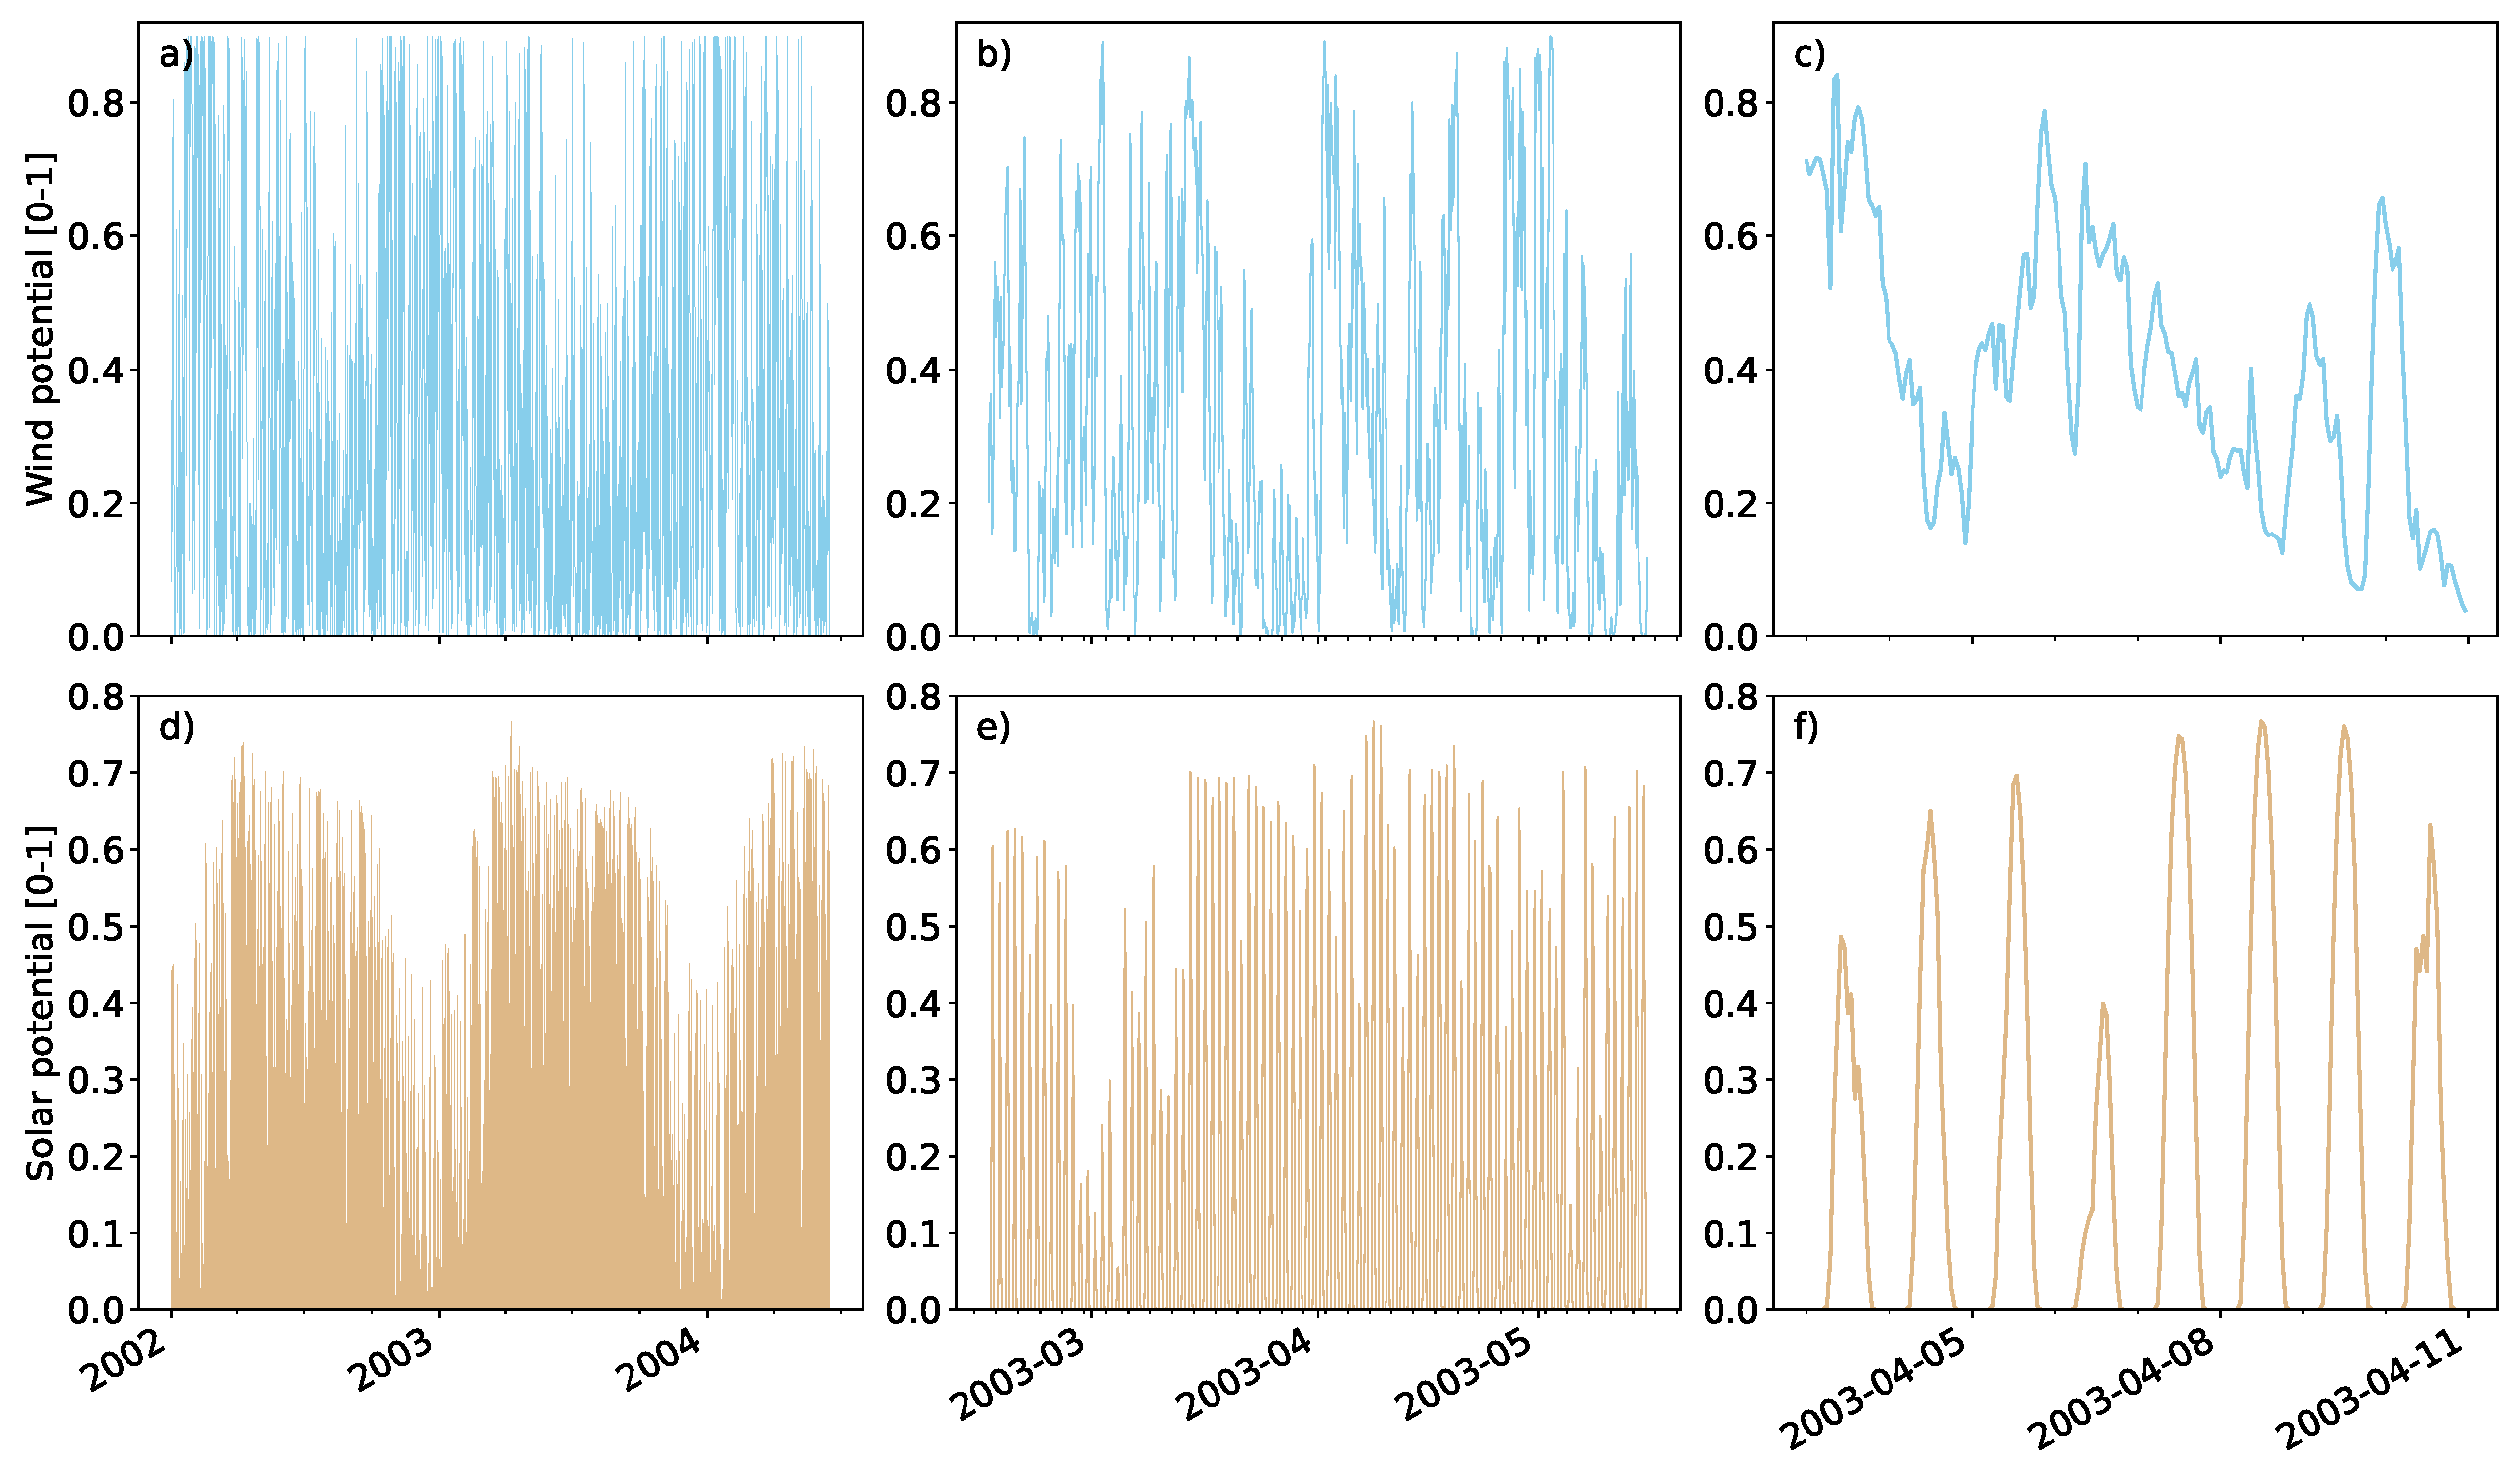
\includegraphics[width=\textwidth]{additional_regions/Climatological_Behaviour_FR10.pdf}
        % 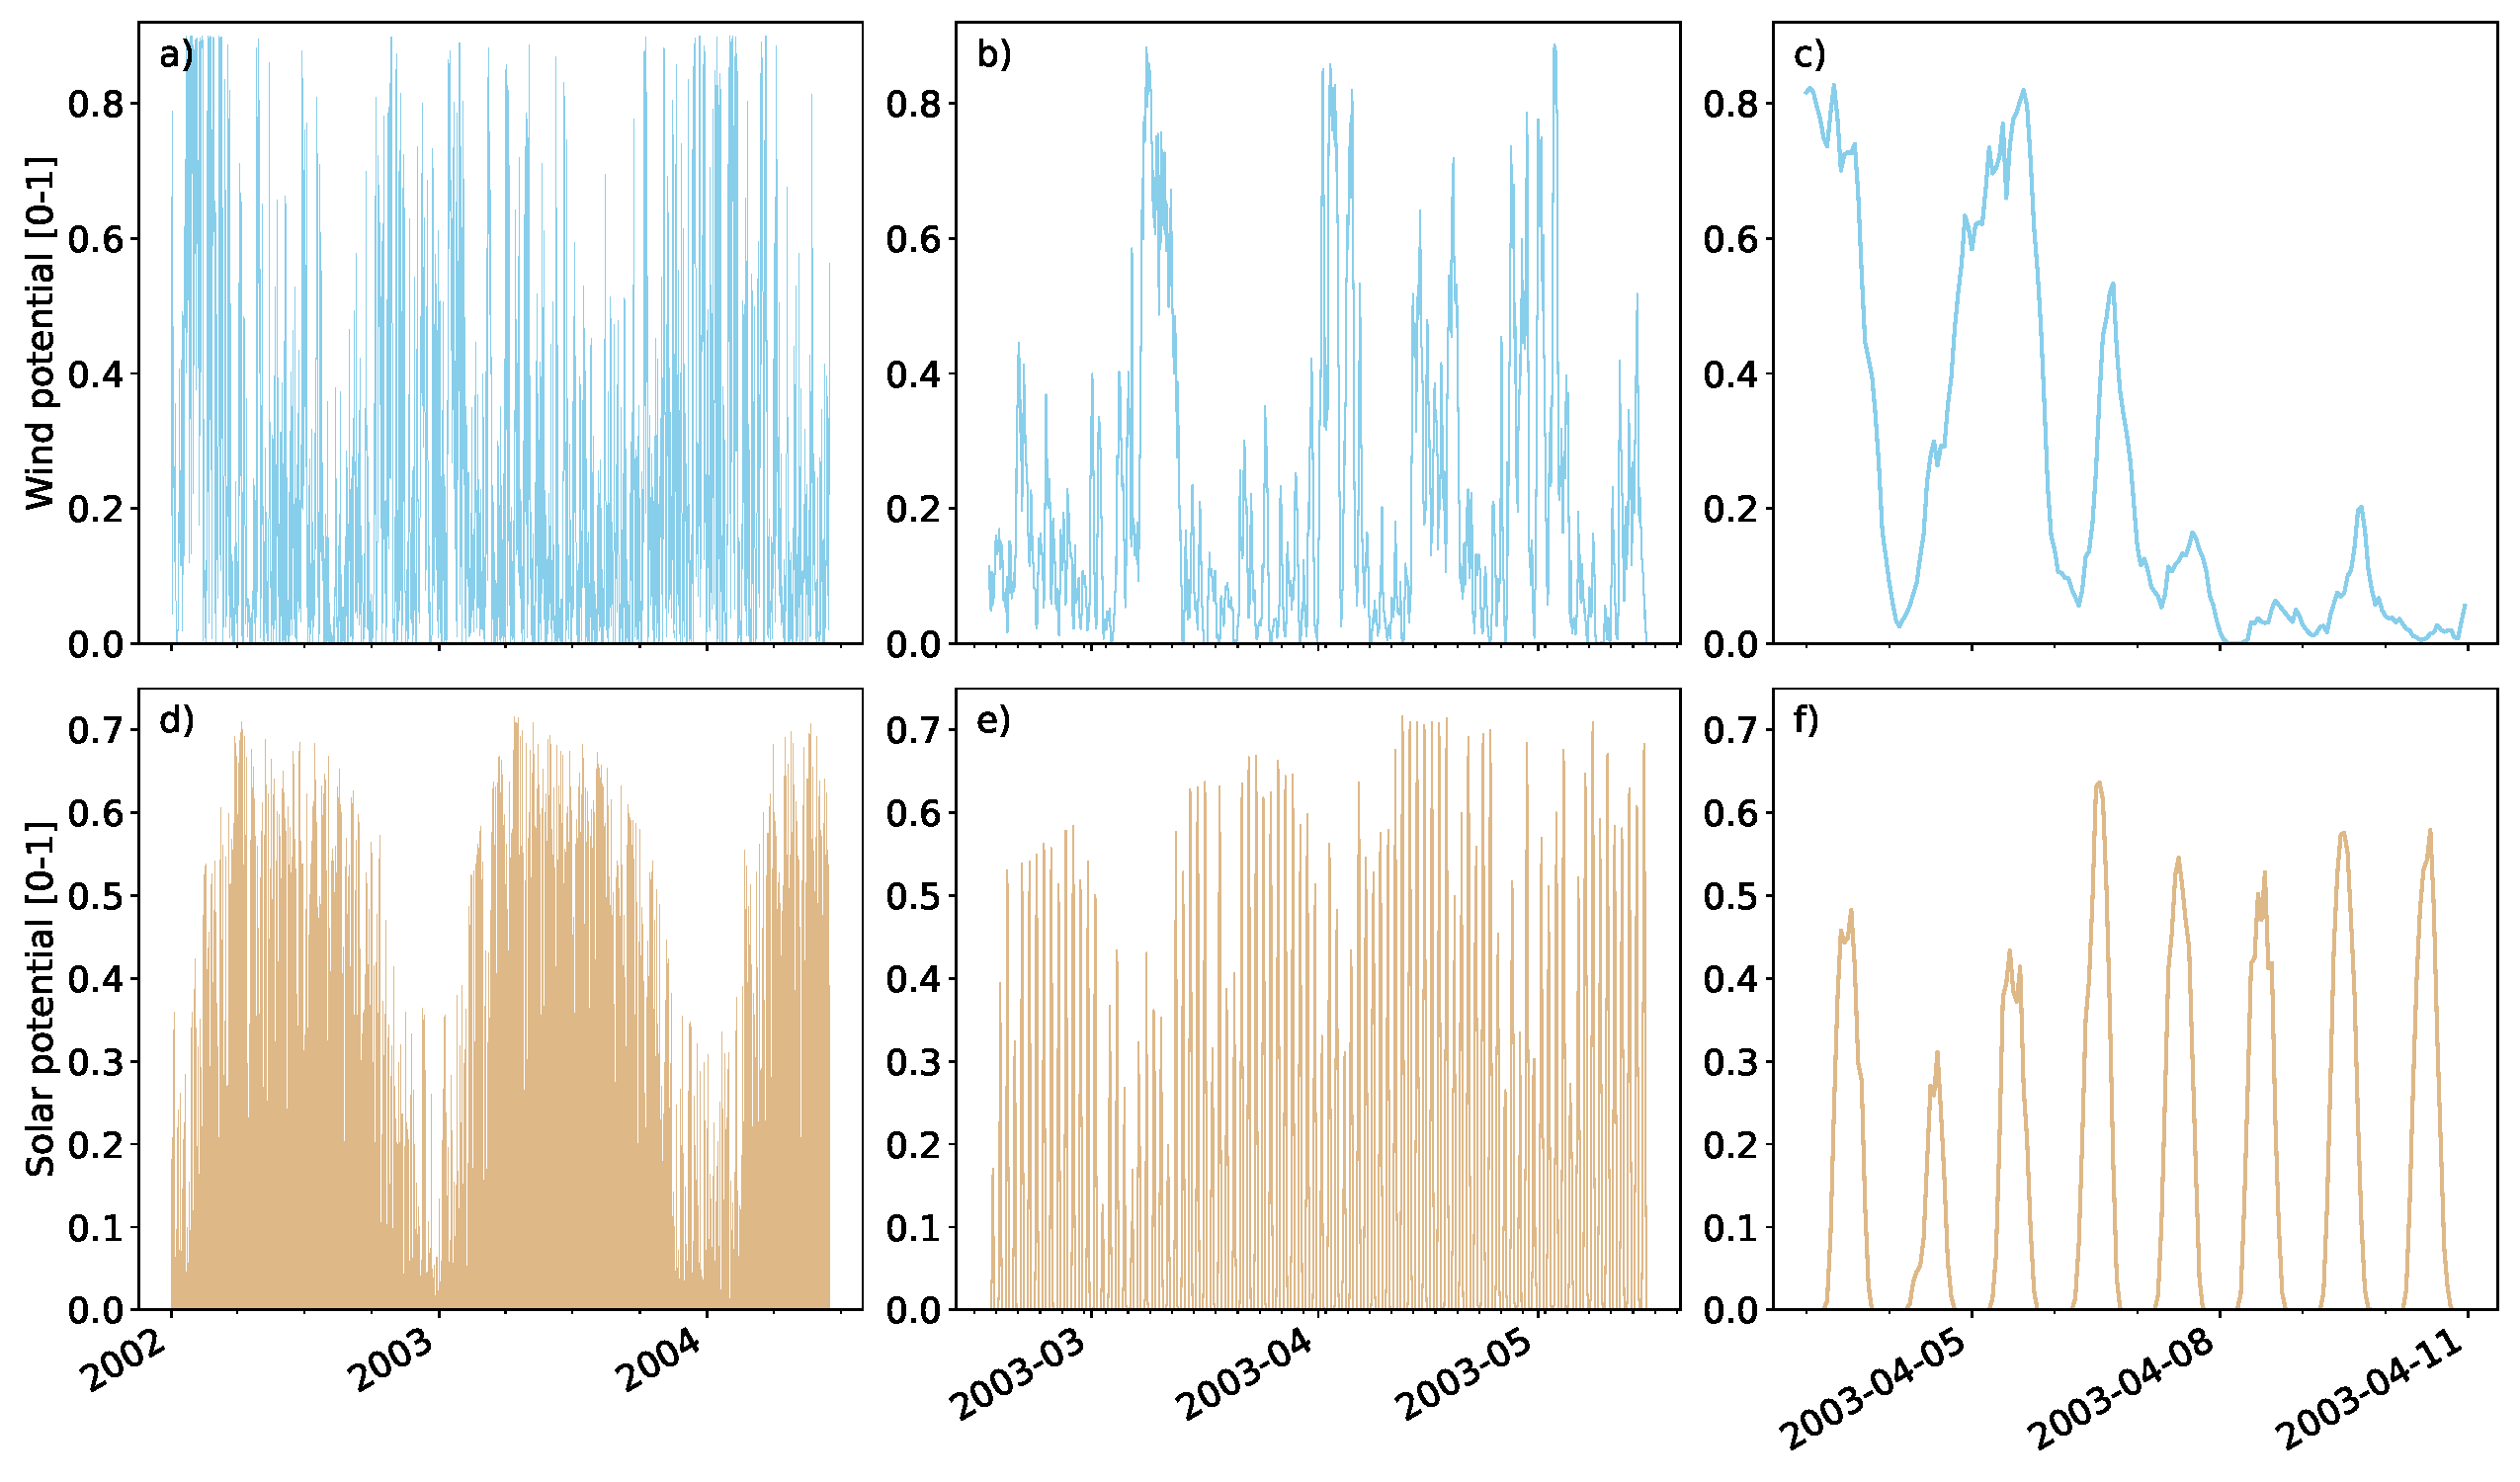
\includegraphics[width=\textwidth]{MainMatter/CP2/Figures/Climatological_Behaviour.pdf}
        \caption{South-East of France (`FR10')}
    \end{subfigure}
    \begin{subfigure}[t]{\linewidth}
        \centering
        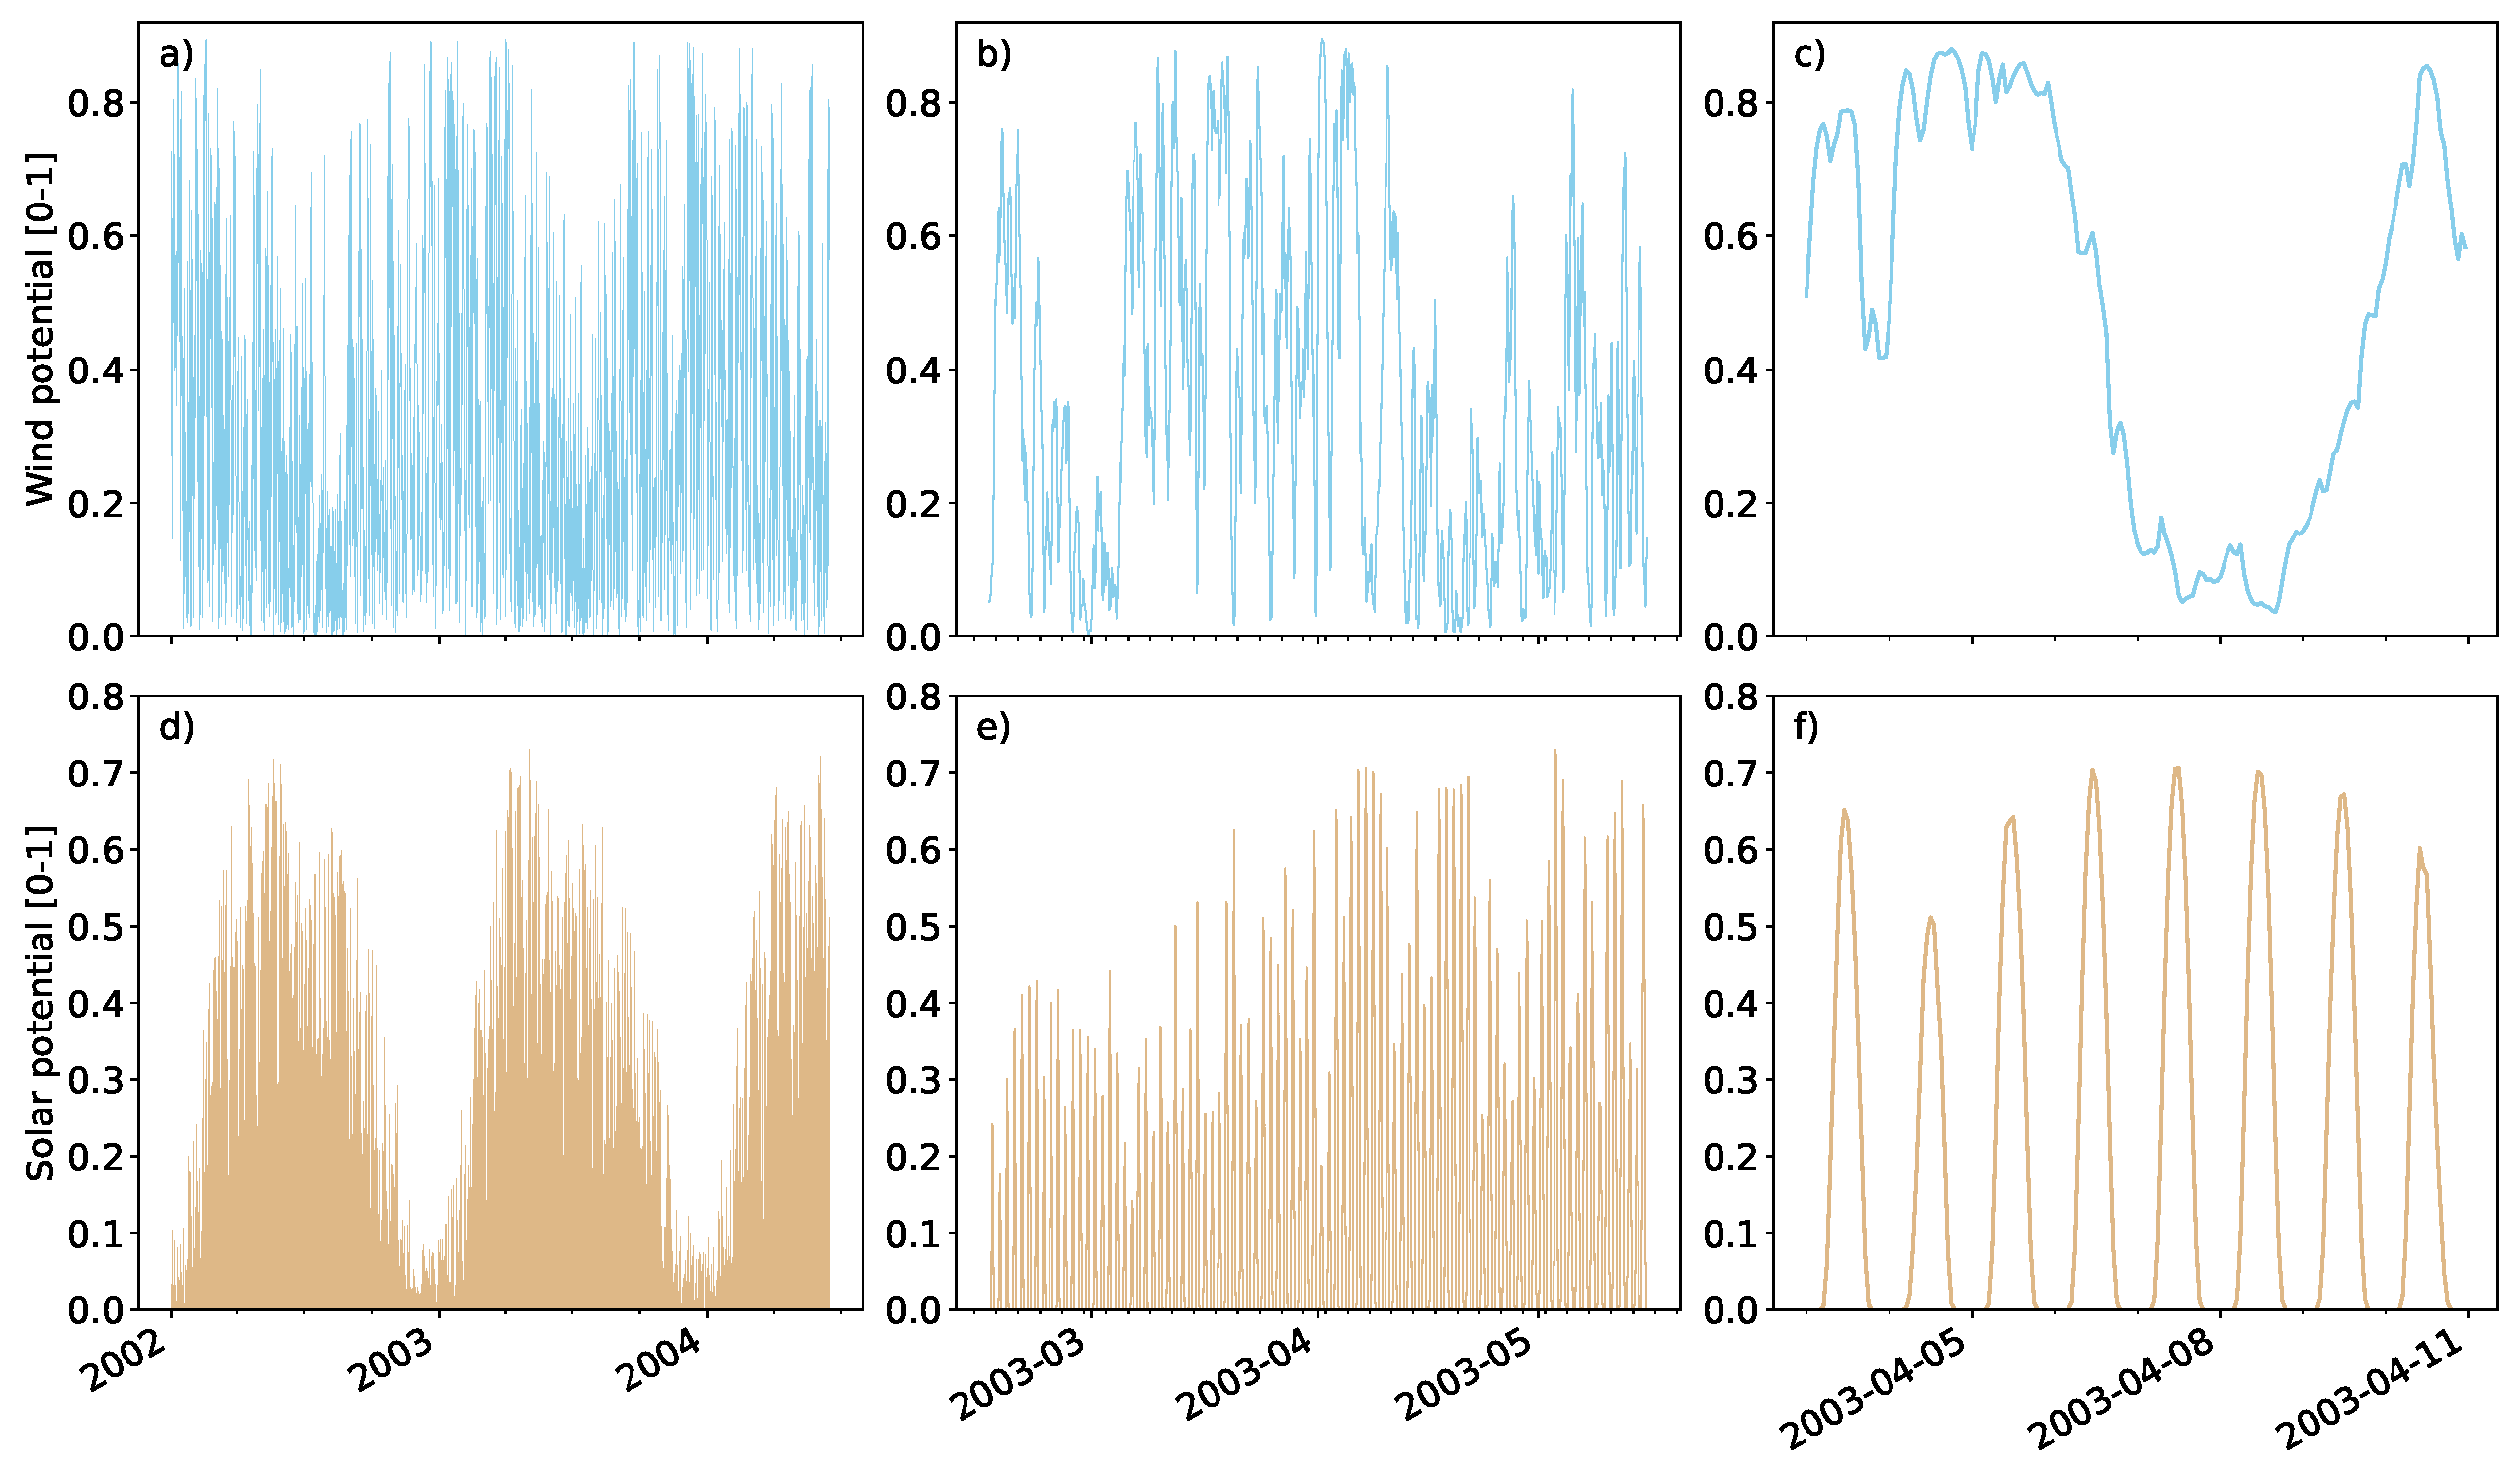
\includegraphics[width=\textwidth]{additional_regions/Climatological_Behaviour_SE02.pdf}
        % 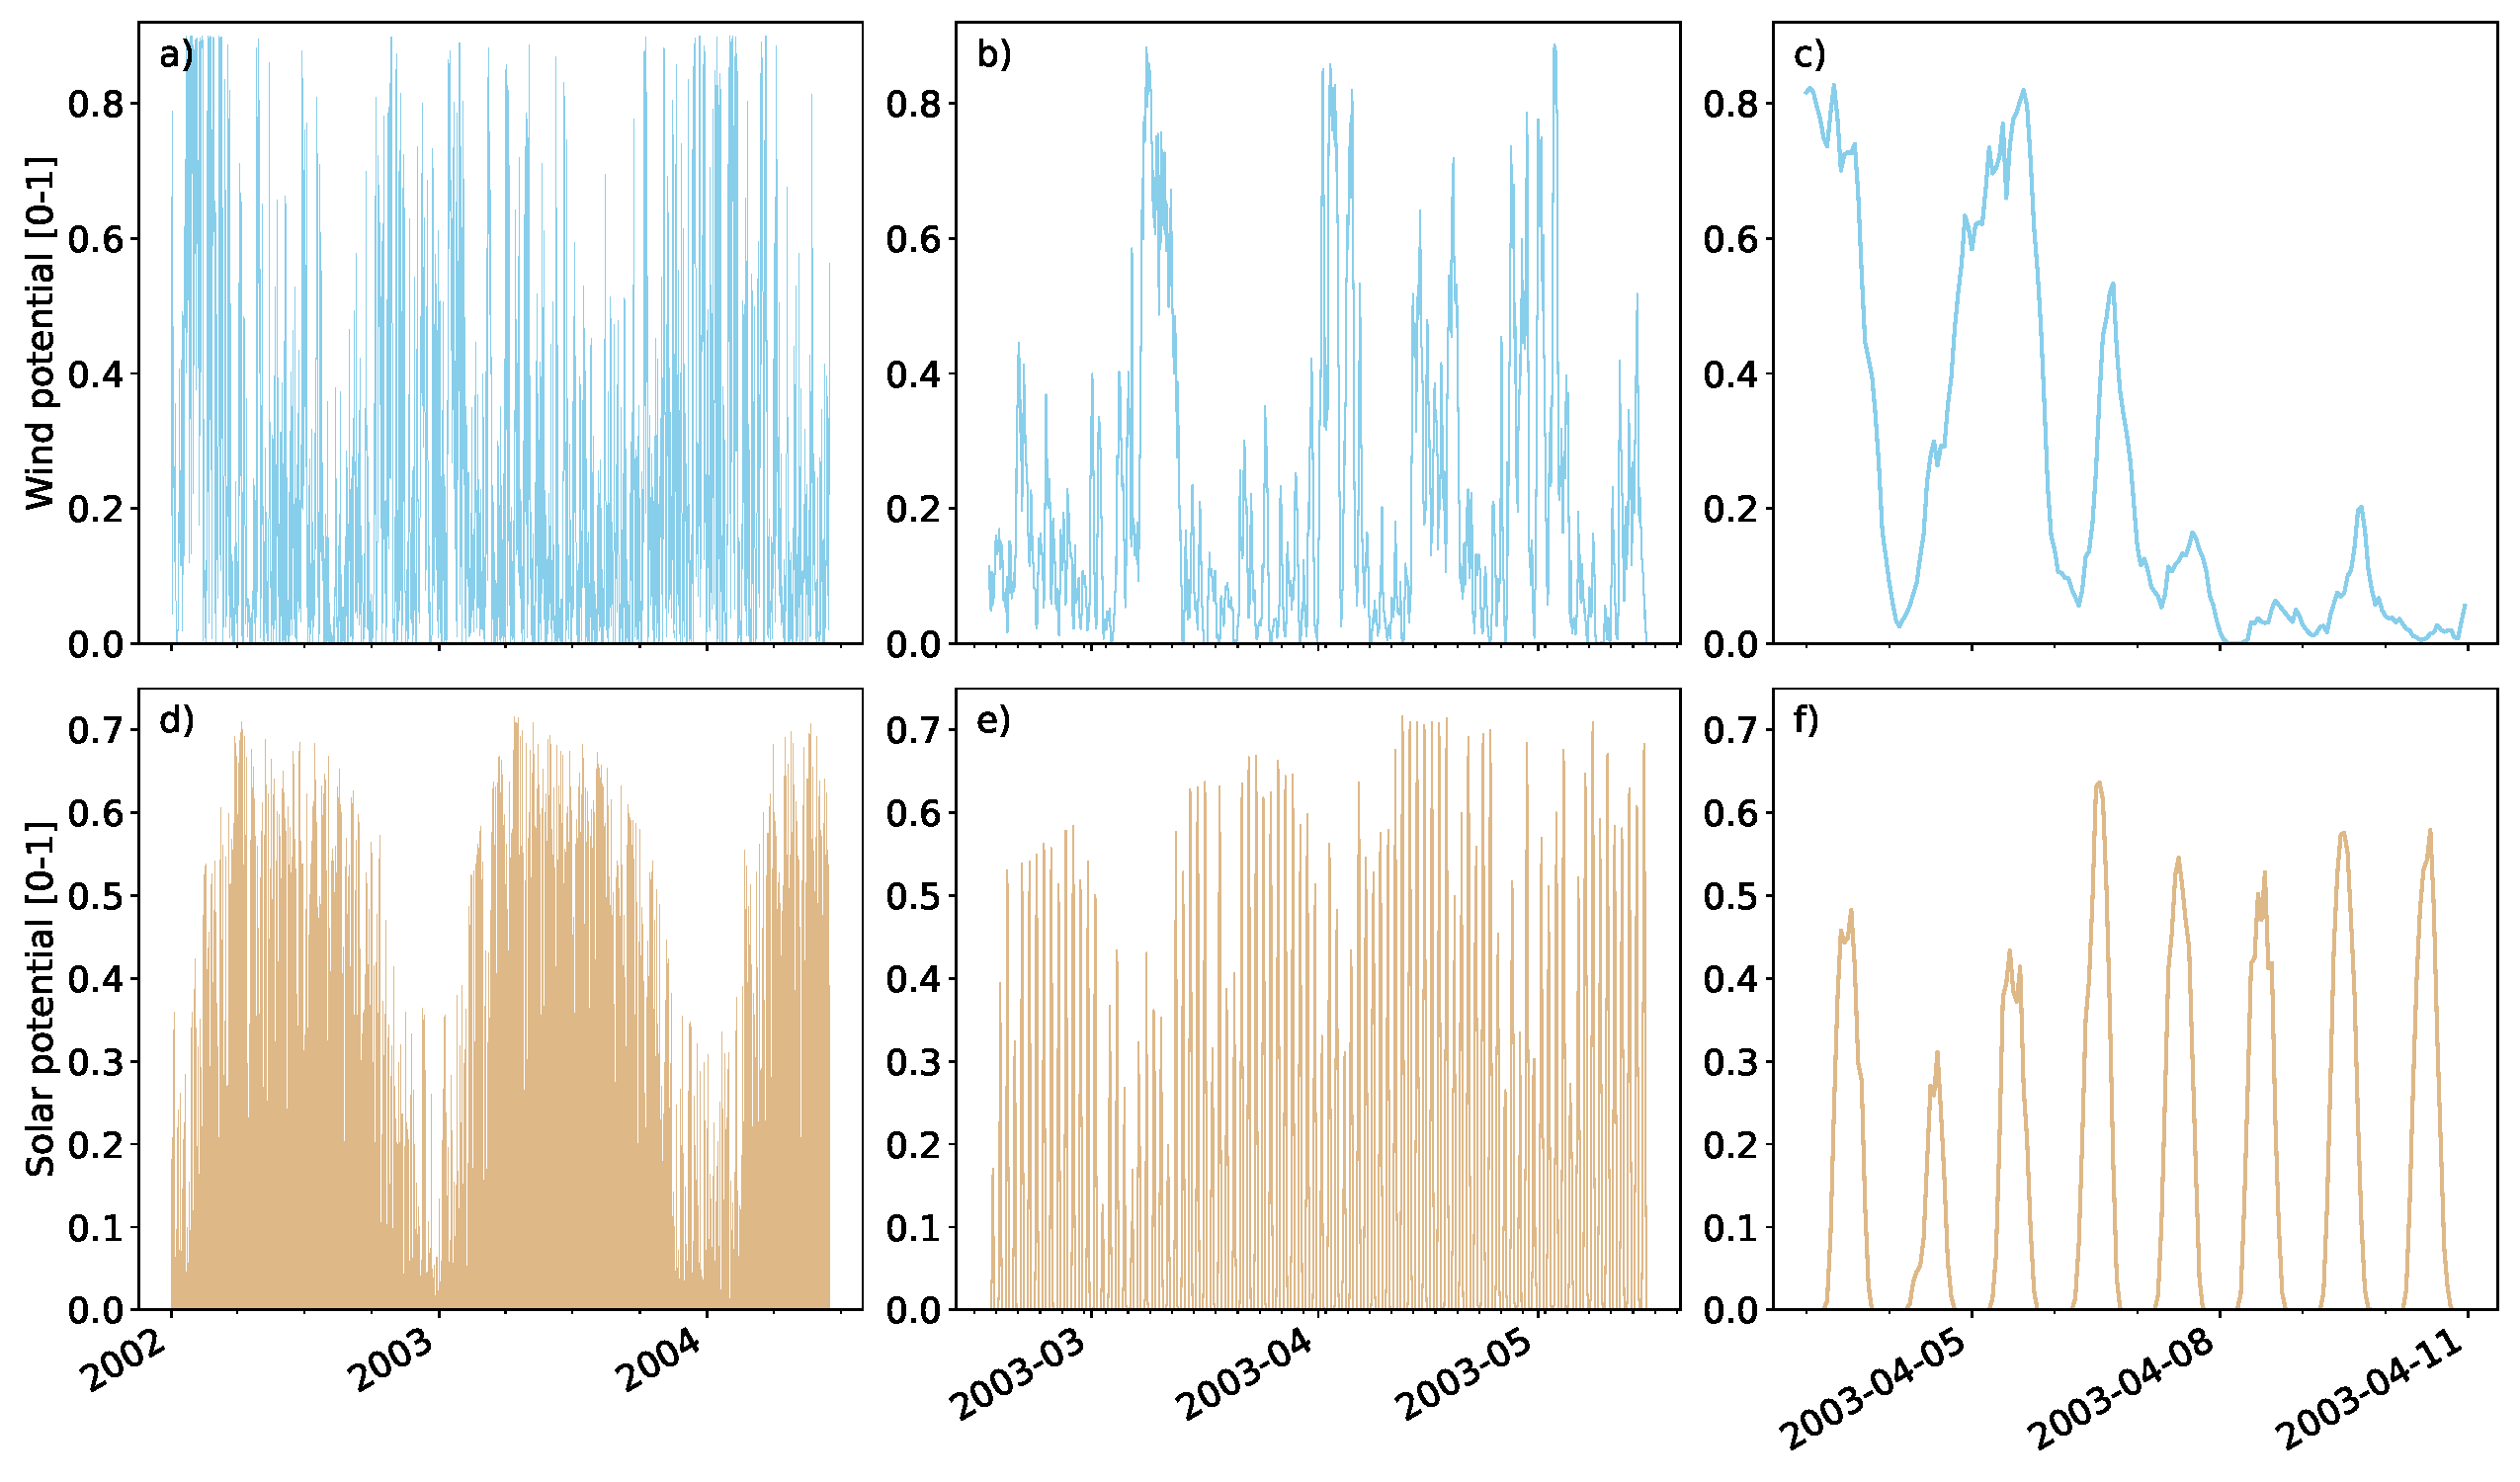
\includegraphics[width=\textwidth]{MainMatter/CP2/Figures/Climatological_Behaviour.pdf}
        \caption{Southern tip of Sweden (`SE02')}
    \end{subfigure}
    \caption{
        As Figure~2 in the main text, but then for the regions as listed for 2002-2004.
        Timeseries of hourly generation potential of wind (top) and solar (bottom). 
        Showing variability on yearly (a,d), sub-seasonal (b,e) and daily (c,f) timescales. 
    }
    \label{SIfig:climatological_behaviour_other-regions}
\end{figure}


\subsection{A hourly rolling windows climate --- Other regions}
% what we show
The \emph{hourly rolling window} climate defined in Section~2.2 of the main text was applied without any changes to the other regions considered.
As can be seen in Figure~\ref{SIfig:climate_other-regions}, this climate provides a smoother description of the expected behaviour on annual timescales and reduces the random fluctuations. 

% observation on the daily wiggle
In line with the observations for the north-west region of the Netherlands, the `initial' climate does capture the annual timescales, but shows random fluctuations from day-to-day and hour-to-hour. 
For both Slovakia and the part of Sweden shown some consistent daily variation is observed for their wind generation potential, whether this is from a physical driver is unknown and should be further studied before using the climatic description for these regions.

\begin{figure}[hb]
    \centering
    \begin{subfigure}[t]{0.9\linewidth}
        \centering
        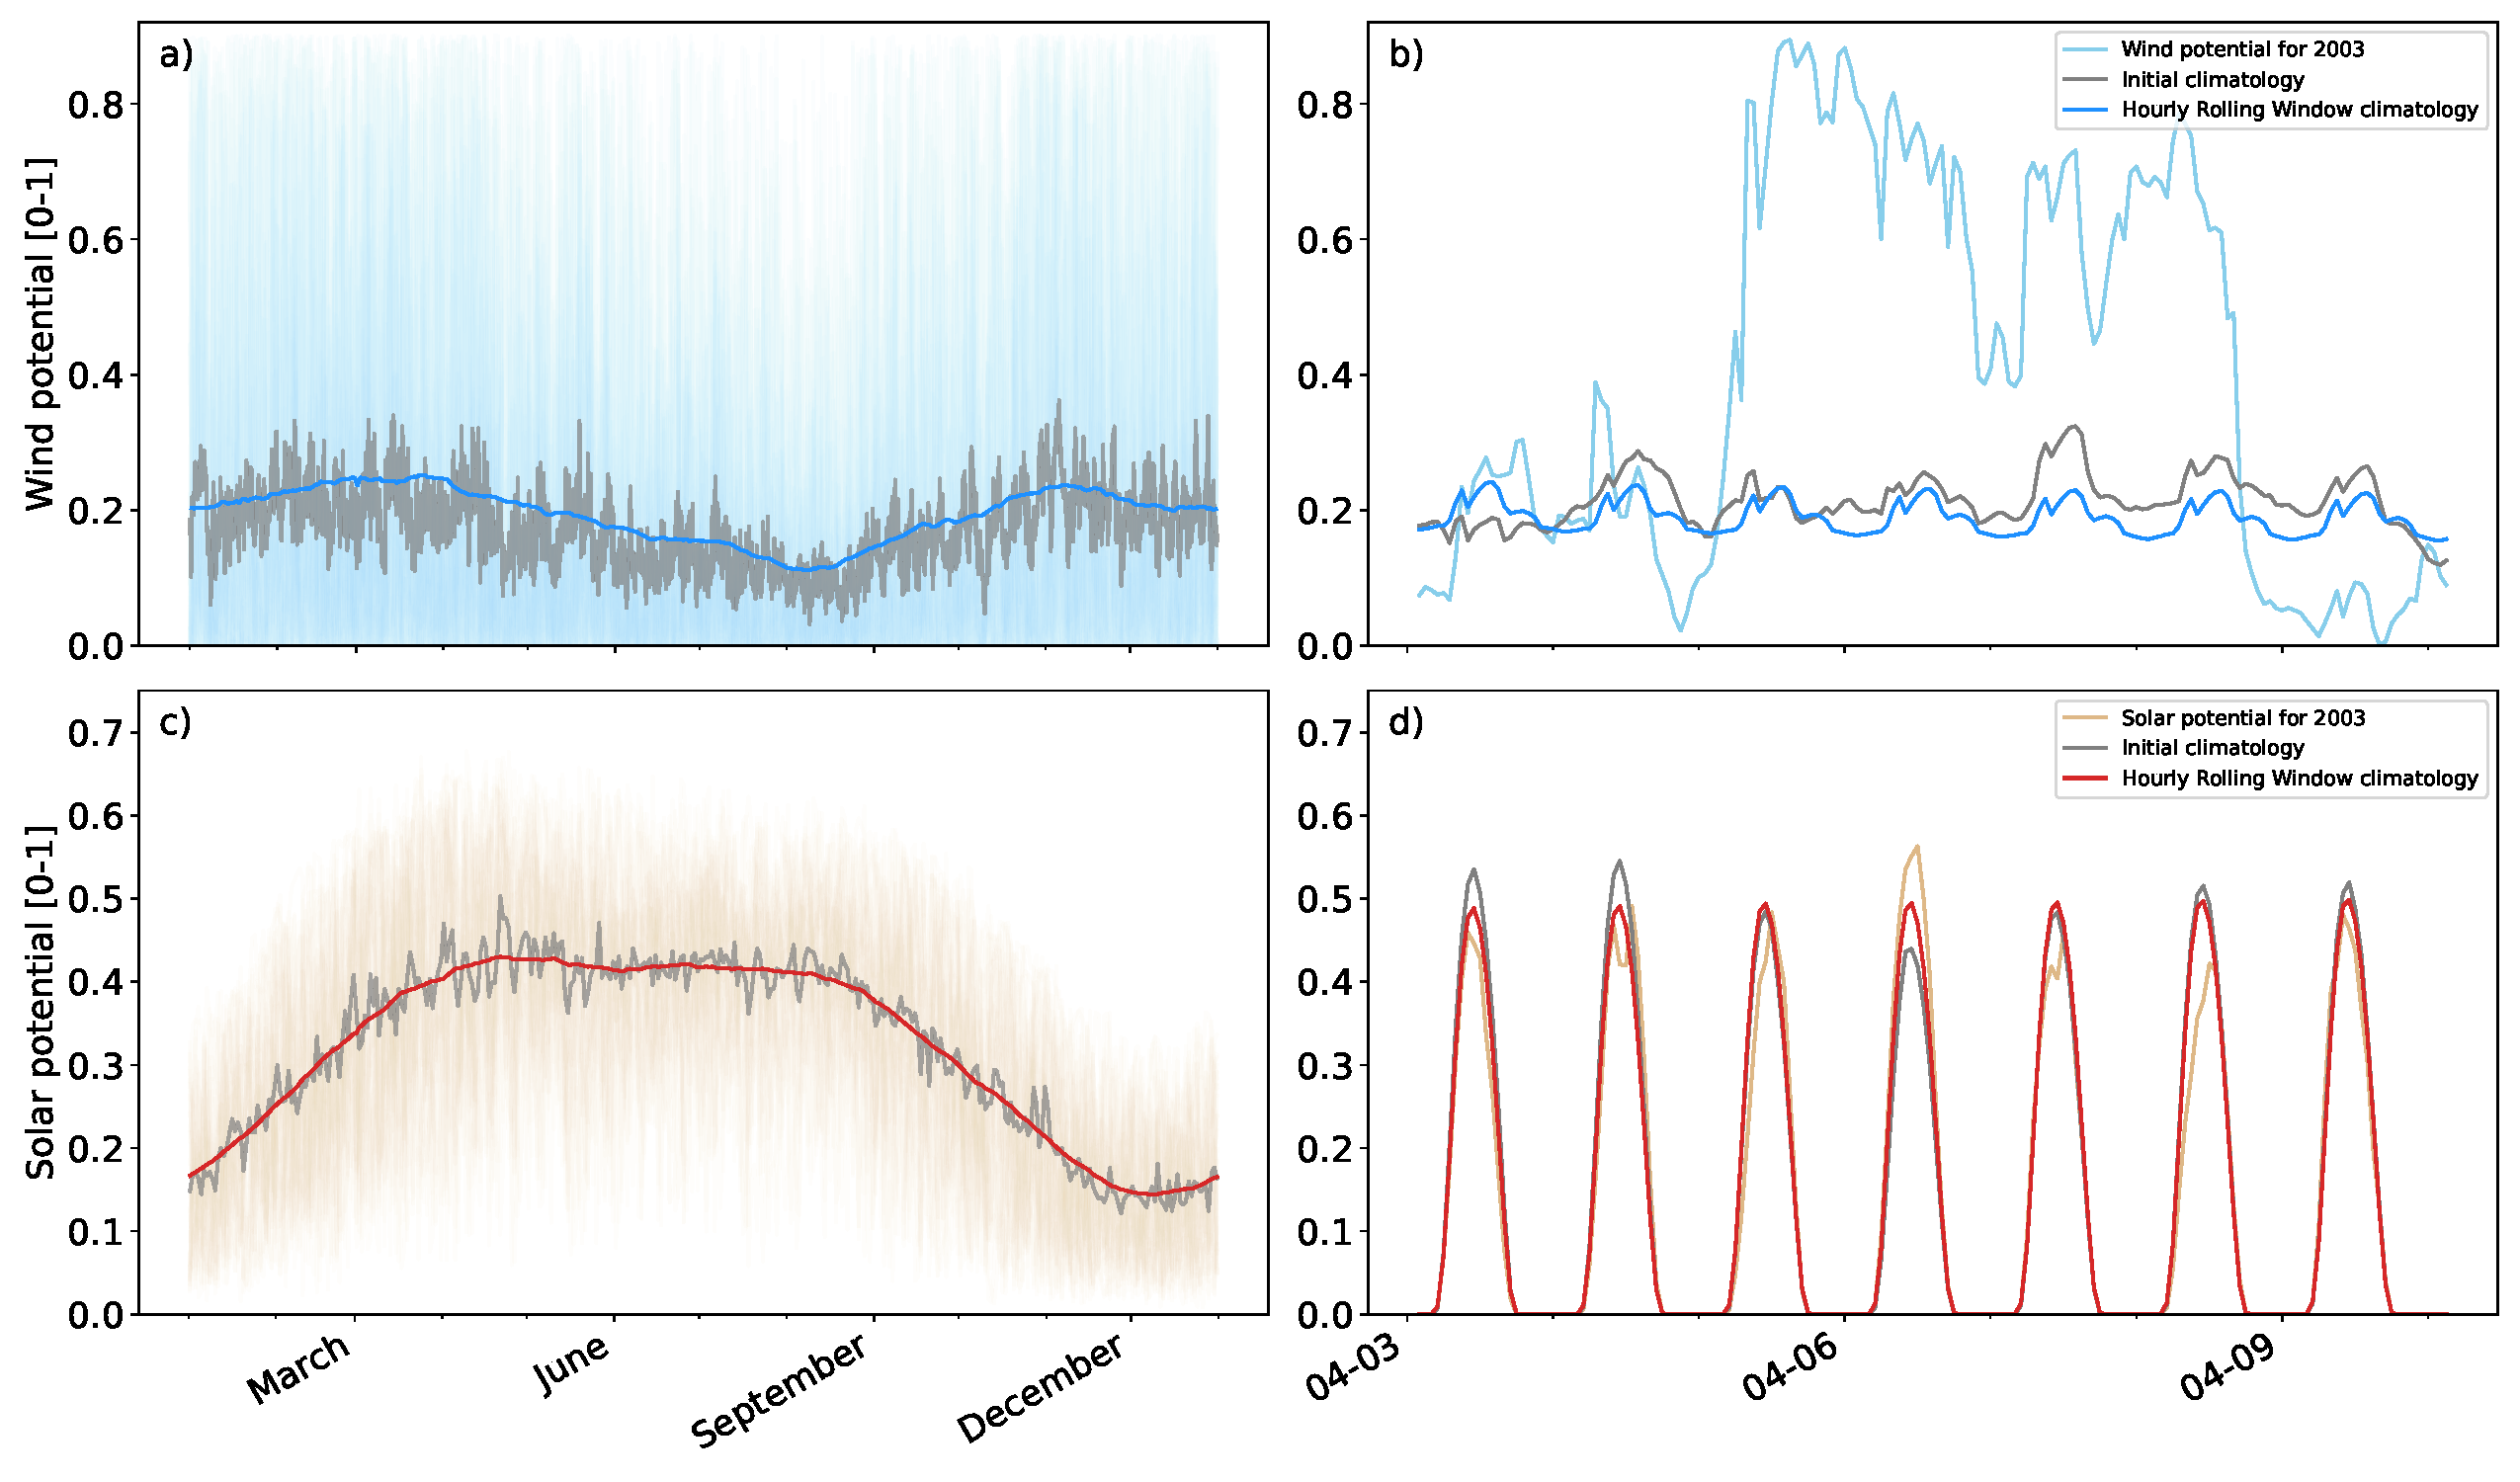
\includegraphics[width=\textwidth]{additional_regions/Climatology_v2_SK00.pdf}
        % \includegraphics[width=\textwidth]{MainMatter/CP2/Figures/Climatological_Behaviour.pdf}
        \caption{Slovakia (`SK00')}
    \end{subfigure}
    \begin{subfigure}[t]{0.9\linewidth}
        \centering
        \includegraphics[width=\textwidth]{additional_regions/Climatology_v2_SE02.pdf}
        % \includegraphics[width=\textwidth]{MainMatter/CP2/Figures/Climatological_Behaviour.pdf}
        \caption{Southern tip of Sweden (`SE02')}
    \end{subfigure}
    \caption{
        As Figure~3 in the main text, but then for the regions as listed.
        Comparison of different methods for computing the climate of the potential generation for wind (top), and solar (bottom), for the period 1991-2020. 
        Figures (a,c) show the hourly generation potentials for each year in this period (light blue for wind and orange for solar), the `initial' climate (grey, see main text for details) and the hourly rolling window climate (blue and red, for wind, solar, respectively). 
        Figures (b,d) show the same, but specifically for the period 3-10 April 2003. 
        For clarity only 13:00 for each day of the year is shown in Figure (c).}
    \label{SIfig:climate_other-regions}
\end{figure}

\clearpage
\subsection{Annual to decadal variability --- Other regions}
% What we show
Section 4.1 in the main text discusses annual to decadal variability observed in the \credi{}, here we shortly discuss the same for other regions. 

% WIND
Over the past 30~years, large and consistent inter-annual variation is observed in the \wdi{} for the `FR10' region (Figure~\ref{SIfig:analysis_decadal_other-regions_A}), while the `SE02' region shows more variable behaviour on annual and seasonal timescales (Figure~\ref{SIfig:analysis_decadal_other-regions_B}).
For the French region, some cumulative effect over the whole period can be observed, while the Swedish region shows a more oscillating pattern. 

% ZON for Solar EB
Similar to the `NL01' region, more inter-annual periods with a flat \sdi{} can be observed then for wind. 
For the French region a general decrease of the \sdi, thus anomalous low generation potential, is observed in the period 1992-2004 and a very consistent increase from 2018 to 2021.
For the Swedish region a yearly flat \sdi{} is observed, likely related to the very limited solar generation potential in the winter. 

\begin{figure}[hb]
    \centering
    \includegraphics[width=\textwidth]{additional_regions/CREDI_interannual_FR10.pdf}
    \caption{
        As Figure~4 in the main text, but then for the South-East of France (`FR10').
        Hourly Wind (a) and Solar (b) \credi{} over the period 1991-2020 for `NL01'. 
        As the climate was calculated over the same period, by definition the \credi{} sums to zero over the full period.}
    \label{SIfig:analysis_decadal_other-regions_A}
\end{figure}

\begin{figure}[ht]
    \centering
    \includegraphics[width=\textwidth]{additional_regions/CREDI_interannual_SE02.pdf}
    % \includegraphics[width=\textwidth]{MainMatter/CP2/Figures/Climatological_Behaviour.pdf}
    \caption{
        As Figure~4 in the main text, but then for the Southern tip of Sweden (`SE02') region. 
        Hourly Wind (a) and Solar (b) \credi{} over the period 1991-2020 for `NL01'. 
        As the climate was calculated over the same period, by definition the \credi{} sums to zero over the full period.}
    \label{SIfig:analysis_decadal_other-regions_B}
\end{figure}

\newpage
\subsection{Seasonal variability --- Other regions}
% What we show
Section 4.2 in the main text discusses seasonal variability in the \credi{}, here we shortly discuss the same for the `SE02' region as it shows the most interesting properties (see Figure~\ref{SIfig:analysis_seasonal_wind_other-regions}). 

% Wind
The \wdi{} in this Swedish region shows similar behaviour as the Dutch region discussed in the main text, but while the 2016 storyline is considered to be the most extreme for the north-west region of the Netherlands, this is not the case for the `SE02' region. 
In addition, the shape of the distribution of the \wdi{} is different throughout the year and the 1996 storyline shows the highest \wdi{} value. 
This stark opposition to the behaviour observed in that storyline for the Netherlands indicates some possible balancing for this specific storyline.

% Solar
The \sdi{} in the southern Swedish region `SE02' shows a very flat value in the period from October to March. 
This is likely due to the very clearly limited solar generation potential in this region during the wintertime period and the reasons for the limited annual to decadal variability observed for this region (see Figure~\ref{SIfig:analysis_decadal_other-regions_B}). 
At the same time large seasonal differences between the different March to September periods are observed. 
As for the `NL01' region, the year 1998 is the most extreme storyline for \sdi.


\begin{figure}[hb]
    \centering
    \begin{subfigure}[t]{\linewidth}
        \centering
        \includegraphics[width=\textwidth]{additional_regions/WindCREDI_annual_SE02.pdf}
        % \includegraphics[width=\textwidth]{MainMatter/CP2/Figures/Climatological_Behaviour.pdf}
        \caption{\wdi{}}\vspace*{0.5cm}
    \end{subfigure}
    
    \begin{subfigure}[t]{\linewidth}
        \centering
        \includegraphics[width=\textwidth]{additional_regions/SolarCREDI_annual_SE02.pdf}
        % \includegraphics[width=\textwidth]{MainMatter/CP2/Figures/Climatological_Behaviour.pdf}
        \caption{\sdi{}}\vspace*{0.5cm}
    \end{subfigure}
    \caption{
        As Figure~5 (here Figure~(a), blue shades) and 6 (here Figure~(b), orange shades) in the main text, but then for the Southern tip of Sweden (`SE02').
        Hourly \wdi{} per analysis year over the period May 1991 to April 2021 for `NL01'. 
        Figure a) shows the specific progression of \wdi{} for each year. 
        Figure b) shows the distribution of the \wdi{} for each hour of the year, namely the 50\ts{th} percentile, the 25-75, 10-90 percentile and min-max range (see legend). 
        Four exemplary storylines are shown, namely 1996 (red), 1998 (green), 2003 (purple) and 2016 (black).
    }
    \label{SIfig:analysis_seasonal_wind_other-regions}
\end{figure}



%%%%%%%%%%%%%%%%%%%%%%%%%%%%%%%%%%%%%%%%%%%%%%%%%%
%%%%		~~~~ Backmatter ~~~~
%%%%%%%%%%%%%%%%%%%%%%%%%%%%%%%%%%%%%%%%%%%%%%%%%%
\clearpage
\ack % Acknowledgement section
Laurens P. Stoop received funding from the  Dutch Research Council (NWO) under grant number 647.003.005. 
The content of this paper and the views expressed in it are solely the author’s responsibility, and do not necessarily reflect the views of TenneT TSO B.V..

\section*{Open research} 
The implementation of the \credi{}, its use at different timescales, all code used to generate the figures, the data from the `NL01' region discussed and the full list of the most extreme short-term events found as presented in this study are available at Github via \url{https://github.com/laurensstoop/ccmetrics} with the MIT license. 

The preliminary data of the PECDv4 containing the regional renewable resource potential for historical technological definitions of wind and solar used for in this study to showcase the \credi{} are not available due to ongoing validation. 
In due time the full PECDv4, including raw gridded and aggregated regional/national renewable resource potentials for a wide range of technological definitions, will be made available as part of the C3S Energy dataset and can be found through \url{https://climate.copernicus.eu/operational-service-energy-sector}. 

% common bib file
\printbibliography 

\end{document}





